\chapter{Unveiling Transcription Factor Dynamics in Cardiac Cells Using Single-Cell RNA-Seq and Epigenomic Data Integration}\thumbforchapter
\chaptermark{Unveiling Transcription Factor Dynamics Using Single-Cell RNA-Seq and Epigenomic Data Integration}

\chapterauthor{Rebecca R. Snabel*, Maarten van der Sande*, Simon J. van Heeringen}
\newpage

\section{Abstract}

Transcription Factors (TFs) bind to specific DNA motifs in cis-regulatory regions and regulate the gene expression of the involved genes. Certain epigenomic assays, such as DNA accessibility and H3K27ac ChIP-seq, coincide with cis-regulatory regions and are used to infer key transcription factor motifs between cell types. RNA-seq, alternatively, measures gene expression and can be used to infer co-expressed regulons and differential transcription factor gene expression. Combining the information in epigenomic and transcriptomic assays greatly improves the discovery of regulatory TFs. Here we present SCEPIA, a computational tool that predicts transcription factor motif activity based on single-cell RNA-seq. SCEPIA works by matching cells to a reference epigenomic database and infers motif activities based on their differential cis-regulatory regions. By correlating these activities to the gene expression of the corresponding TFs, SCEPIA is able to infer differential regulation of TFs between cells. We confirm the accuracy of the inferred motif activities by SCEPIA through a multiomic re-analysis of the Human Heart Cell Atlas. In conclusion, SCEPIA is a computational tool that improves motif activity inference based on single-cell RNA-seq, and is freely available at \url{https://github.com/vanheeringen-lab/scepia}.

\section{Introduction}

The gene activity of a cell is shaped by a complex network of interacting genes, with a special role reserved for transcription factors (TFs). TFs selectively bind to specific DNA sequences (motifs) in accessible cis-regulatory DNA and interact with other nearby transcription factors or recruit co-activators\cite{Spitz2012}. These co-activators chemically modify histone tails, where different modifications are associated with specific regulatory roles. The H3K27ac modification loosens the histone-DNA association, which in turn makes DNA more accessible\cite{Creyghton2010}. More accessible DNA exposes new motifs, which allows for new TFs to bind to regulate gene expression\cite{Tsompana2014}. Thus, to understand transcription regulation, it is crucial to consider the interaction between cis-regulatory regions and transcription factors\cite{Xu_2020,Kamal_2021,Gonz_lez_Blas_2022,Fleck2022,Kamimoto2023,Kartha2022}. The interactions between TFs, cis-regulatory regions, and their target genes are generally represented and studied as a gene regulatory network (GRN).

Single-cell sequencing has emerged as a rapidly expanding field, allowing researchers to explore the gene expression and epigenomic profiles of mixtures of cell types. One of the earliest methods to infer GRNs based on single-cell transcriptomics is the method SCENIC\cite{Aibar_2017}. SCENIC matches TFs and target genes based on co-expression, and filte interactions based on TF motifs in cis-regulatory regions in proximity of the TSS of the target gene. Whilst co-expression based networks can be insightful, they suffer from spurious interactions, as transcript abundance correlates poorly with protein count\cite{Fortelny2017,Franks2017}, can not measure post-translational modifications, and ignore chromatin context. As a consequence, single-cell multiomics GRN inference methods such as Pando\cite{Fleck2022}, SCENIC+\cite{Gonz_lez_Blas_2022}, CellOracle\cite{Kamimoto2023}, and FigR\cite{Kartha2022} have been introduced. These multiomic-based methods leverage the chromatin context by determining TF and target gene interactions based on the motifs present in accessible regions and use the level of DNA accessibility as a proxy for regulatory ability. Although multiomic sequencing assays are immensely valuable, they remain costly and generate sparser data compared to their single-cell transcriptomics and bulk epigenomic counterparts\cite{Li2021}. Given the fact that the information between epigenomic and transcriptomic assays partially overlaps\cite{Wang2016,GonzlezRamrez2021}, the opportunity arises for computationally matching gene expression profiles with (bulk) epigenomic assays of similar cell types. 

Here we explore the question of whether transcription factor motif activity inference from single-cell gene expression data can be improved by linking to an independently obtained epigenomic reference. This approach has two advantages. First, single-cell RNA-seq is cheaper and more straightforward to perform in many cell types than single-cell epigenomic or multiomic assays (e.g. scATAC, scCUT\&Tag, 10X Multiome). Second, by linking these assays one effectively obtains multiomic data. This, in turn, allows for improved motif activity inference, by linking motif activities with gene expression and ultimately removing spurious interactions. We call this approach Single-cell EPigenome-based Inference of Activity (SCEPIA). Based on an analysis of  [....], we demonstrate SCEPIA's ability to identify key transcriptional regulators of cardiac cell types (i.e. \textit{GATA4}, \textit{TBX5}, \textit{FLI1} and \textit{RUNX1}). Furthermore, this approach was previously shown instrumental in uncovering \textit{Onecut2} as a regulator of M-cells in intestinal organoids\cite{LunaVelez2023}. With SCEPIA, we present a new methodological approach to uncover transcription regulators from single-cell transcriptomic data. 

\section{Results}

\subsection{Accurate motif activities through a reference epigenomic database}

We hypothesized that incorporating a measure of cis-regulatory element activity, such as ATAC-seq or H3K27ac ChIP-seq, would be beneficial to identify transcription factor motif activity from single-cell transcriptomic data, even when this activity is not experimentally measured in the same experiment. Here, we used the regulatory potential to match single-cell RNA-seq profiles to a collection of predetermined H3K27ac ChIP-seq profiles. The regulatory potential is defined as the weighted average H3K27ac signal per gene \cite{Wang2016}. To determine how well regulatory potential specifically matches RNA-seq data for identical cell types, we obtained data from 96 human RNA-seq cell types and 121 human H3K27ac cell types from ENCODE\cite{encode_dcc}. We calculated the regulatory potential for all H3K27ac samples, and computed the correlation coefficient for all combinations of regulatory potential and RNA-seq values (Fig. \ref{fig:bulk_comparison}A). In general, the regulatory potential shows only a high positive correlation for a subset of the transcriptomic data, indicating that the measure captures cell type-specific signals. The mean correlation coefficient for identical cell types between regulatory potential and transcripts per million (TPM) was found to be 0.53 with a standard deviation of 0.14. In 64\% of the H3K27ac experiments, the regulatory potential of a given cell type exhibited the highest correlation with the TPM of the same cell type. Furthermore, in 77\% of the cases, the highest correlation was observed with a tissue sharing the same ontology term (UBERON ontology for tissues, Cell Line ontology for primary cells, and cell lines are not mapped to an ontology term). As noted previously\cite{Wang2016}, the specific parameters used for calculating regulatory potential do not significantly impact the results. For this specific analysis, the H3K27ac signal in the promoter region (2kb up- and downstream of the TSS) alone is sufficient to predict the TPM (Table \ref{table:correlations}). In summary, our findings suggest that a collection of H3K27ac regulatory potential can effectively serve as a reliable classifier for characterizing cell states based on transcriptomic data.

\begin{figure}
    \centering
    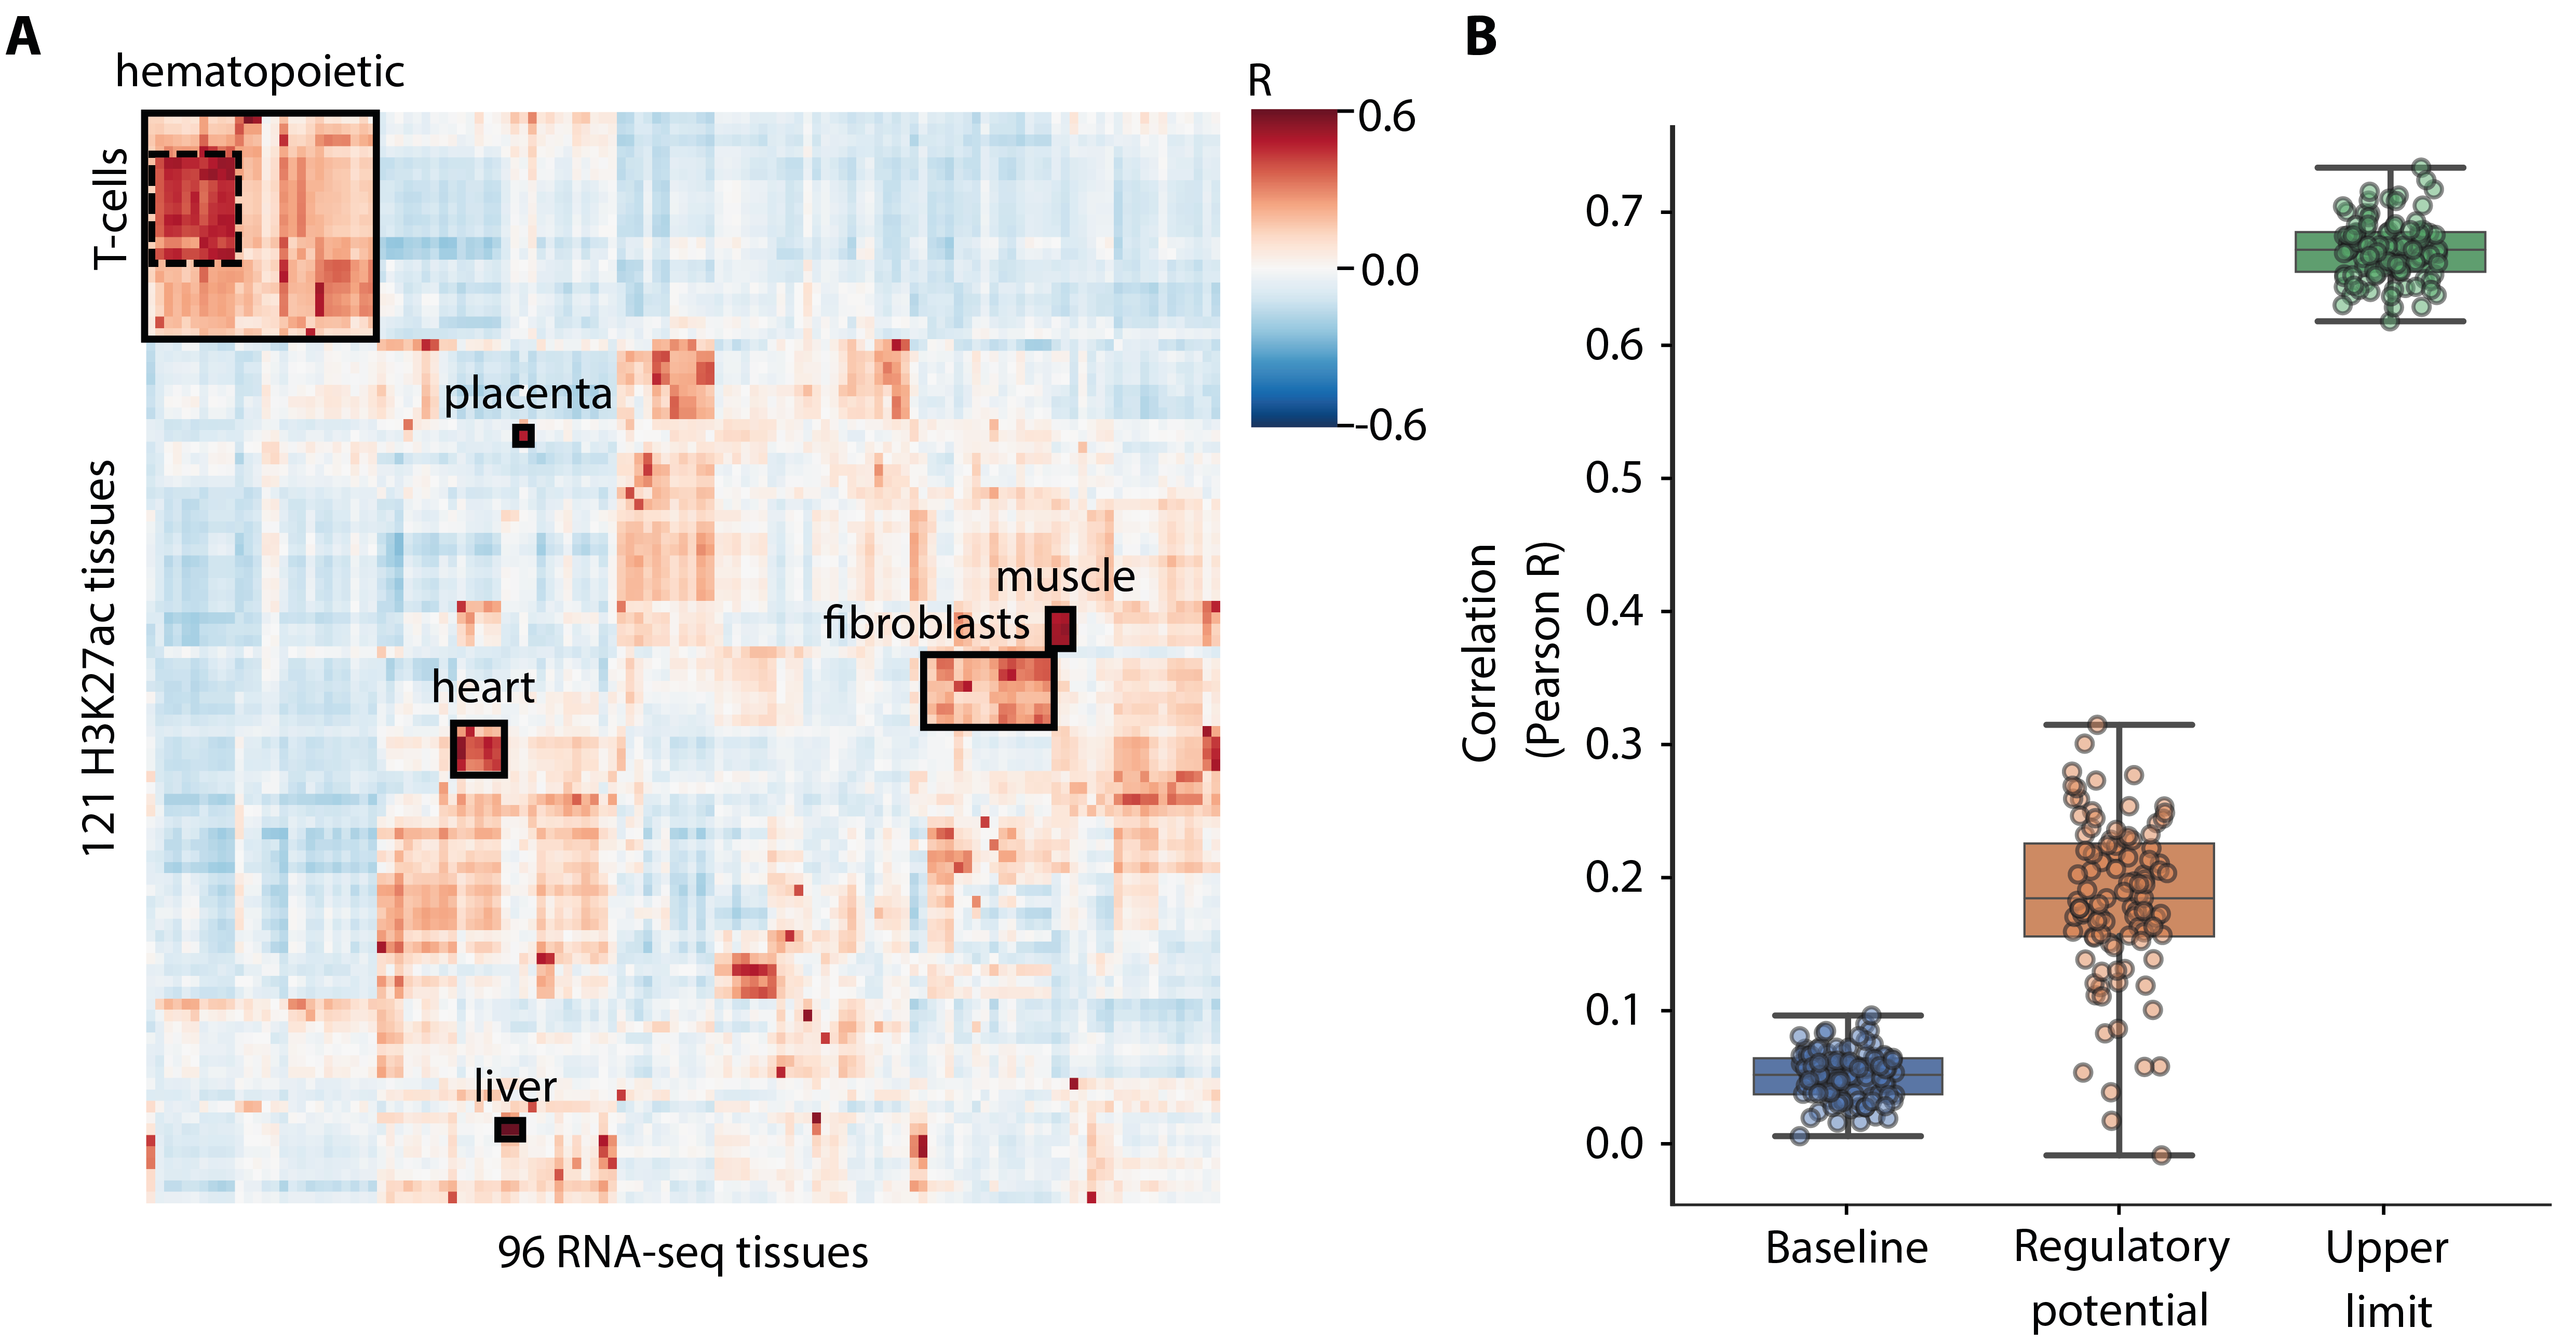
\includegraphics[width=1\linewidth]{ch.scepia/imgs/CellTypes_MvS_Myriad_thicks_Figure1.png}
    \caption{\textbf{Automatically matching epigenomic information to transcriptomic data improves motif activity inference.} \textbf{(A)}: The Pearson correlation coefficients between all combinations of regulatory potential of 121 H3K27ac cell types and TPM values of 96 RNA cell types. Rows and columns are hierarchically sorted, which clusters similar cell types in proximity, for example, the hematopoietic, heart, and muscle cells. \textbf{(B)}: Regulatory potential-based motif activities are superior to the baseline based on transcriptomic data alone. The motif activities of 5 random cell types are inferred based on the H3K27ac signal in the top 25,000 differential enhancers (100 permutations). The baseline approach to motif activity inference with only transcriptomic data is to assume that the TPMs of transcription factors are identical to their motif activity (mean correlation of 0.04). The regulatory potential-based approach automatically matches transcriptomic samples to H3K27ac samples in a hold-out set. It infers the motif activity scores on their top 10,000 differential enhancers (mean correlation of 0.17). Finally,  the upper limit evaluates the effect of the size of the enhancer set, and compares the inferred motif activities between enhancer sets the size of 10,000 and 25,000 (mean correlation of 0.66).}
    \label{fig:bulk_comparison}
\end{figure}

In general, the H3K27ac signal in regulatory sequences can be used to determine motif or transcription factor activity\cite{FANTOM2009,Balwierz2014,Madsen_2017}. This motif activity, which quantifies the contribution of each motif to H3K27ac peak strength, is a powerful measure of the relevance of a transcription factor for a specific cell state. The relationship between RNA-seq and regulatory potential led us to assume that transcription factor motif activity can be inferred from transcriptomic data, through an intermediate collection of matched H3K27ac data. As the reference collection contains a limited number of cell types, an exact matching cell type may not always be available for a specific cell type measured by RNA-seq. Therefore, we decided to calculate a composite measure of motif activity, based on a combination of reference cell types (see Methods). To calculate this measure, we regressed the TPM values of the 2,000 most variable genes of a collection of cell types against our regulatory potential database. From there, we selected the top 50 cell types based on the absolute regression coefficients and identified the top 10,000 most differentially enriched cis-regulatory regions within these 50 cell types. Subsequently, we calculated the motif activity using these enhancers and obtained the final motif scores by taking the dot product of motif scores and regression coefficients. 

To test the accuracy of this method, we made one hundred random subsets of five tissues common to both our H3K27ac reference database and transcriptomic dataset. Our first step involved establishing a ground truth for motif activities by conducting a motif scan on the top 25,000 most differentially enriched cis-regulatory regions within each of these five tissues. Here, these regions were defined based on a union of all public transcription factor binding peaks, as obtained from the ReMap database\cite{Chneby2017} (see Methods). As a baseline approach to estimating motif activity based solely on transcriptomic data, we assumed a direct one-to-one translation between the transcripts per million (TPM) values of a transcription factor and its motif score. However, as Figure \ref{fig:bulk_comparison}B illustrates, this baseline approach displays a particularly poor correlation with our ground truth (mean correlation of 0.04). Instead, our approach based on regulatory potential demonstrates a significantly improved correlation (mean correlation of 0.17). It is important to note that the cell types used for the ground truth are excluded from the reference database. Finally, to assess the sensitivity of our approach to the choice of cis-regulatory region set, we compared the ground truth data based on the top 25,000 most variable regions with that based on the top 10,000 most variable regions. Taken together, these analyses show that RNA-seq can be reliably matched to H3K27ac in a cell type-specific manner and that this data can be used to estimate transcription factor activity in a more reliable manner than gene expression alone. See supplemental figure \ref{fig:bulkbenchmark} for a one-factor-at-a-time parameter sweep, which shows that the results of SCEPIA are robust across a wide range of settings.

\subsection{SCEPIA accurately annotates single-cell populations and identifies known cardiac regulators}

We showed the possibility of matching cell type-specific H3K27ac-inferred regulatory potential to an RNA-seq dataset. SCEPIA was set up to incorporate this principle into single-cell transcriptomic analysis. Figure \ref{fig:scepia_overview}) shows a schematic overview of SCEPIA and individual steps are explained in more detail in the Methods. In short, the gene expression levels per cell type are inferred from the promoter accessibilities of the reference data and this inferred expression is used to match with the provided single-cell query to annotate the cells (steps 1 \& 2). From the top 50 highest-ranking cell types in the annotation, the 10,000 most variable peaks are used to perform motif scanning (step 3). The cell type-annotation weights are used to determine single-cell motif activities (step 4), and by correlating motif activity and TF expression, the best TF-motif match is established (TF activity; step 5). Finally, in this last step, the significance of the hits is determined by permutation testing on randomized data. To evaluate performance, we conducted a comparative analysis on a multimodal dataset from the human Heart Cell Atlas v2 (hHCA; \cite{Kanemaru2023},) which encompasses over 700,000 cells profiled by scRNA-seq and spans the different anatomical regions and cellular subtypes of the human heart. We ran SCEPIA on the single cell transcriptomic assay of this atlas and used various strategies to evaluate the different steps incorporated in SCEPIA (Fig. \ref{fig:scepia_overview}). First, we ran SCEPIA on all cells of the atlas to asses its overall performance. We checked the intermediate outcomes of the run, such as the ability to annotate the cell type of the single cells correctly with the H3K27ac reference (outcomes of steps 1 \& 2), as well as the inference of regulatory factors of importance (outcome of steps 3-5). 

\begin{figure}
    \centering
    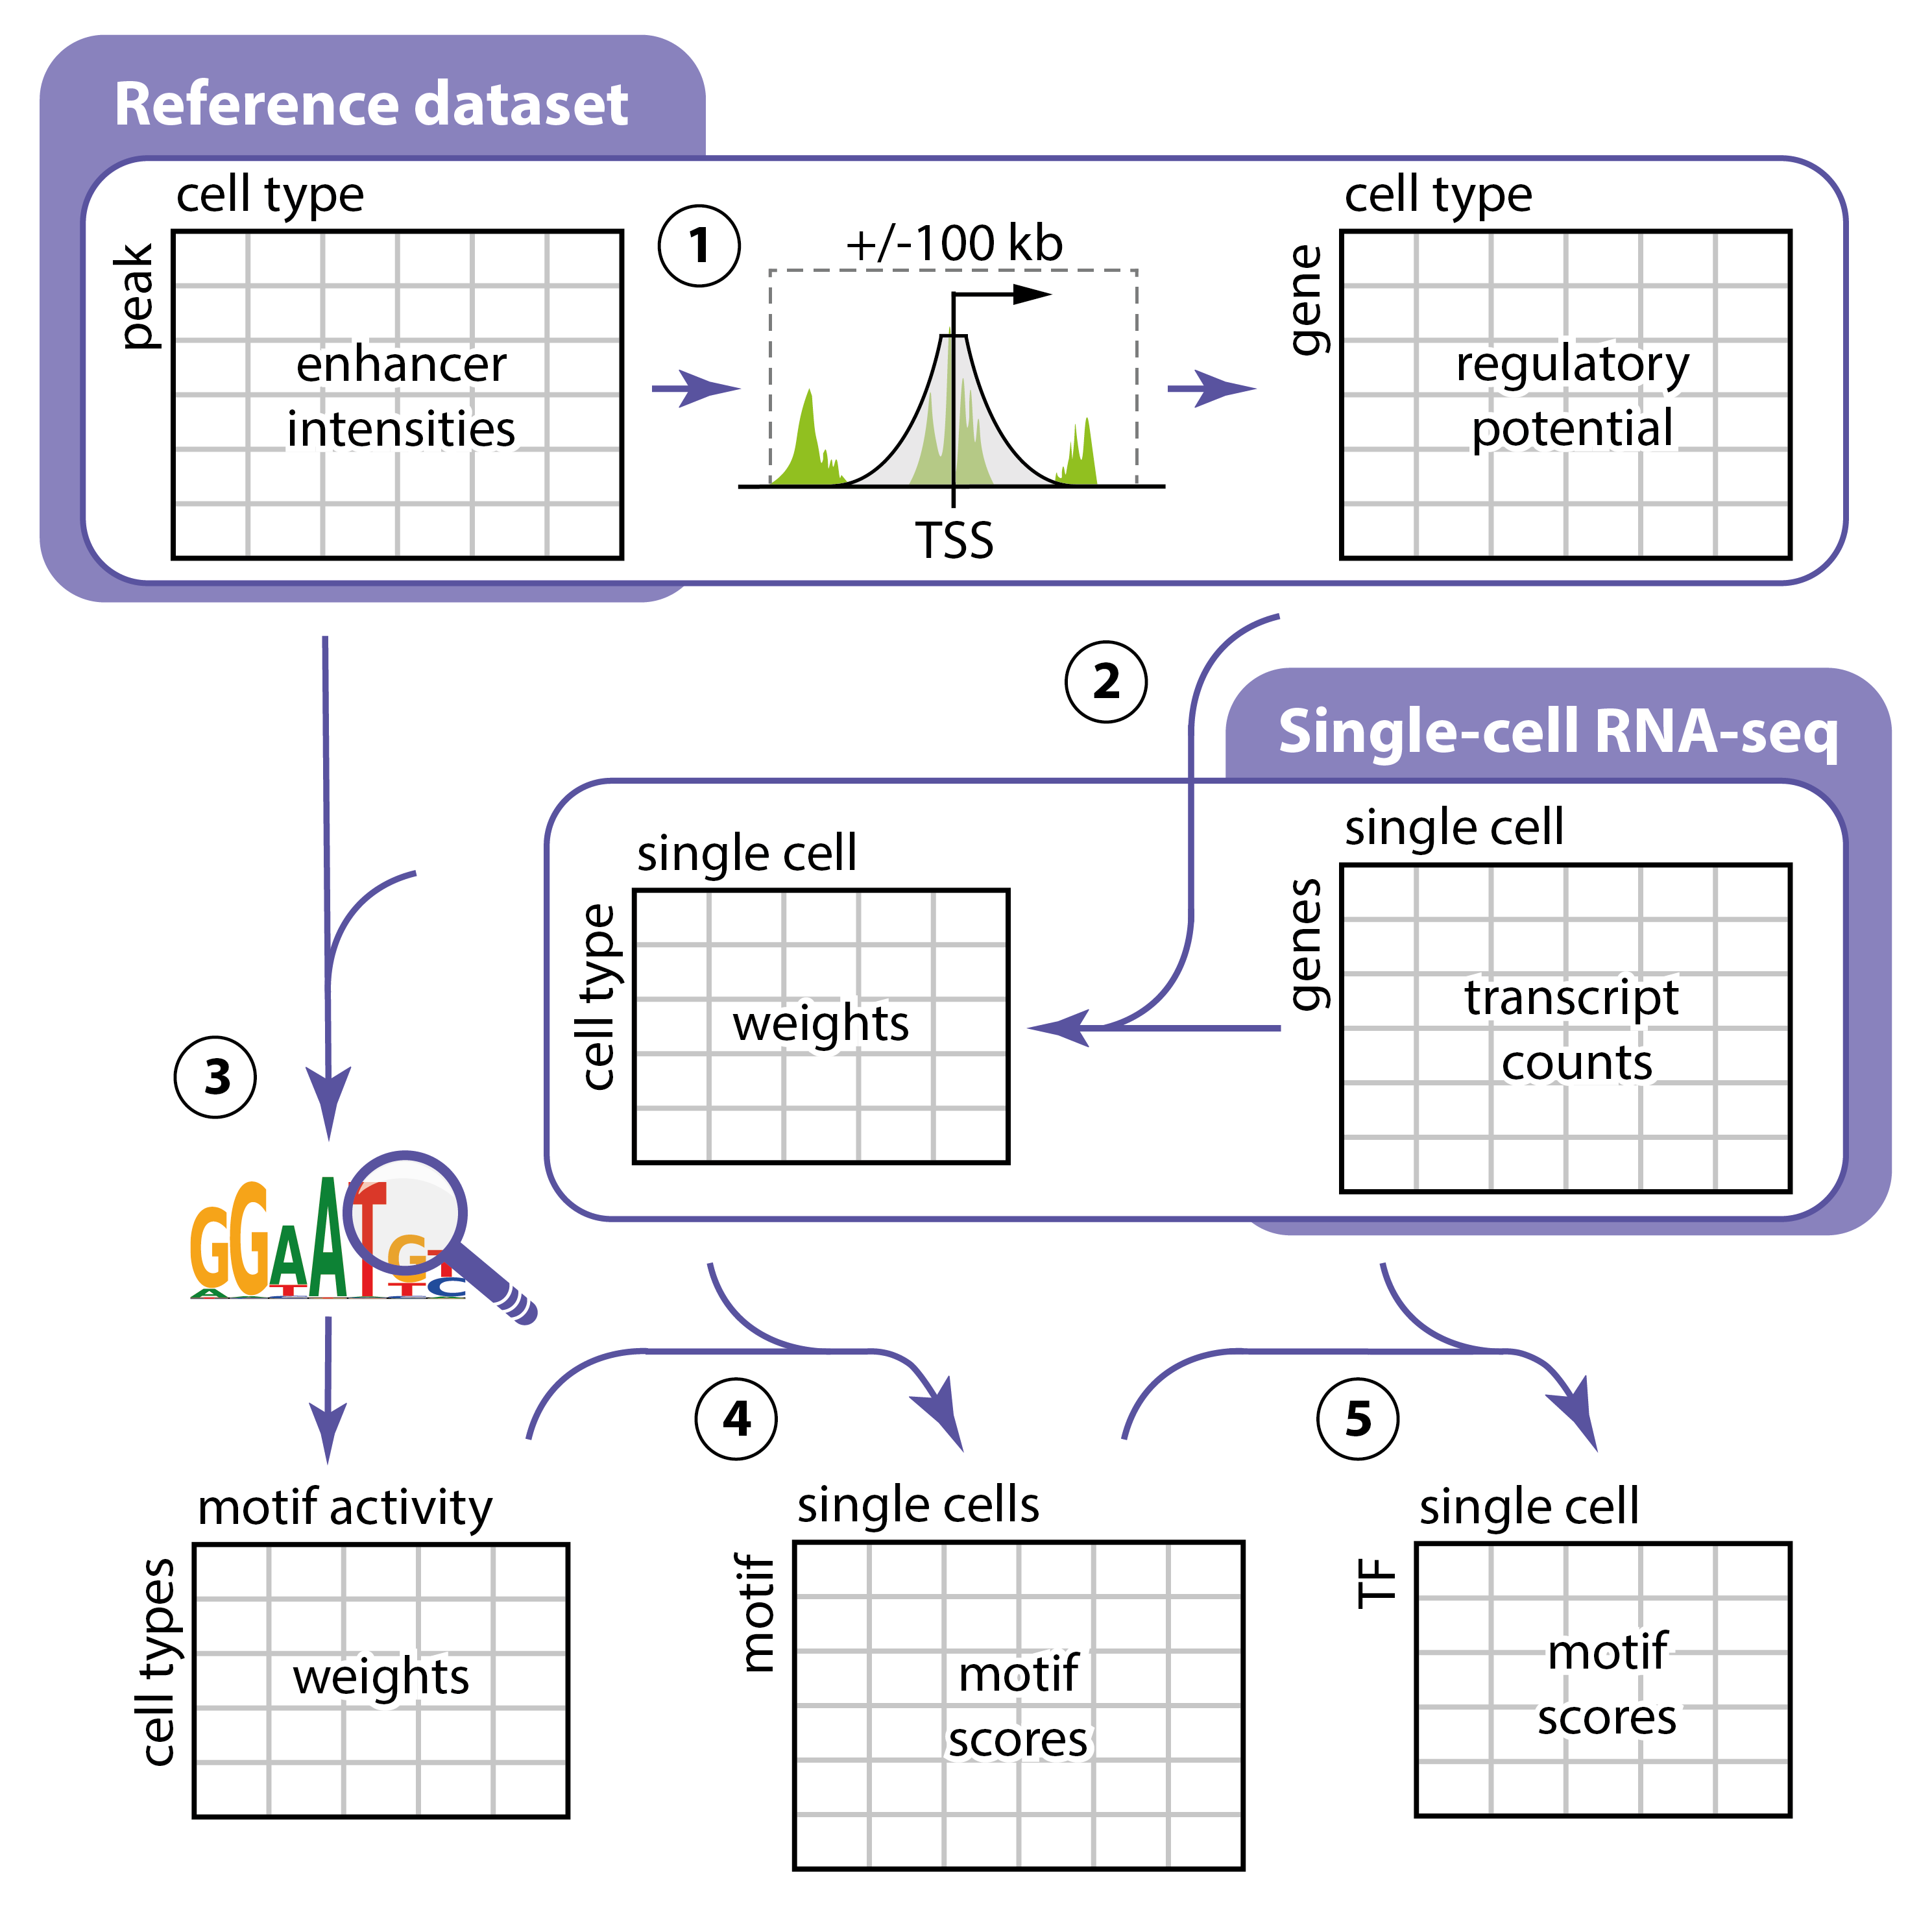
\includegraphics[width=0.95\linewidth]{ch.scepia/imgs/OverviewFigure_SvH_Myriad_v6_Figure2.png}
    \caption{\textbf{Overview of Single-Cell EPigenome-based Inference of Activity (SCEPIA).} See the methods for an extensive explanation per step. \newline 
    \textbf{Step 1}: Calculate the regulatory potential from distance-weighted chromatin assay intensities around each gene for each cell type in the reference collection.
    \textbf{Step 2}: Regress the single-cell gene expression on the regulatory potential. Keep the top 50 cell types with the absolute highest regression coefficients to use as the cell type weights for each cell.
    \textbf{Step 3}: Select the top 10,000 most differential enhancers between the top 50 cell types, and use them for motif activity inference.
    \textbf{Step 4}: Take the dot product between the motif activities and the cell type weights, resulting in motif activities for each motif per cell. Motif activities are scaled to a motif score between 0-1. 
    \textbf{Step 5}: Calculate the correlation coefficient between the expression level (log2 TPM) and the motif activity for TF-motif pairs. A permutation test between gene expression and motif activities allows for the estimation of the statistical significance of their relation.}
    \label{fig:scepia_overview}
\end{figure}

Accurate annotation of cell types by SCEPIA is important (Fig. \ref{fig:scepia_overview}: Step 2), as all subsequent analyses rely on this initial step. We demonstrated that this matching is accurate for bulk RNA-seq data (Fig. \ref{fig:bulk_comparison}A). To validate if matching of the reference also works on single-cell data, we compared the inferred annotation of SCEPIA (Figure \ref{fig:scepia_hhca1}) with the cluster annotation as provided by the HCA authors (Figure \ref{fig:scepia_annotation1}). SCEPIA correctly assigned the atrial and ventricular cardiomyocyte clusters to heart ventricle and cardiac atrium, respectively. The fibroblasts, neural cells and mural cells (i.e. smooth muscle cells or pericytes of the vasculature), all matched to tissues or cell types similar to their identity, albeit originating from a different organ or tissue (i.e. lung or tibia) (Figure \ref{fig:scepia_hhca1}A). Similarly, the myeloid and lymphoid clusters were matched with cell types from the correct major immune lineage branches, namely CD14+ monocytes and CD8+ T cells, respectively. SCEPIA had more difficulty annotating the endothelial cells, which showed the best match with heart left ventricle and a comparatively weaker match to umbilical vein endothelial cells (Fig. \ref{fig:scepia_annohm}). This may be attributed to the high prevalence of endothelial cells in the heart myocardium, as also evident from the cluster size of the endothelial cells in the atlas. Ultimately, in the analysis by SCEPIA, the endothelial cluster was represented by a combined signature of heart left ventricle and an endothelial cell type. Likewise, the adipocytes are represented by a mixed signature of right cardiac atrium and adipose tissue (Figure \ref{fig:scepia_annohm}). For the mesothelial cluster, there was no matching cell or tissue type available in the ENCODE database, which could explain the lack of any strong matches for this cluster. Overall, these findings highlight that SCEPIA matched the majority of the clusters correctly to the ENCODE reference. 

\begin{figure}
    \centering
    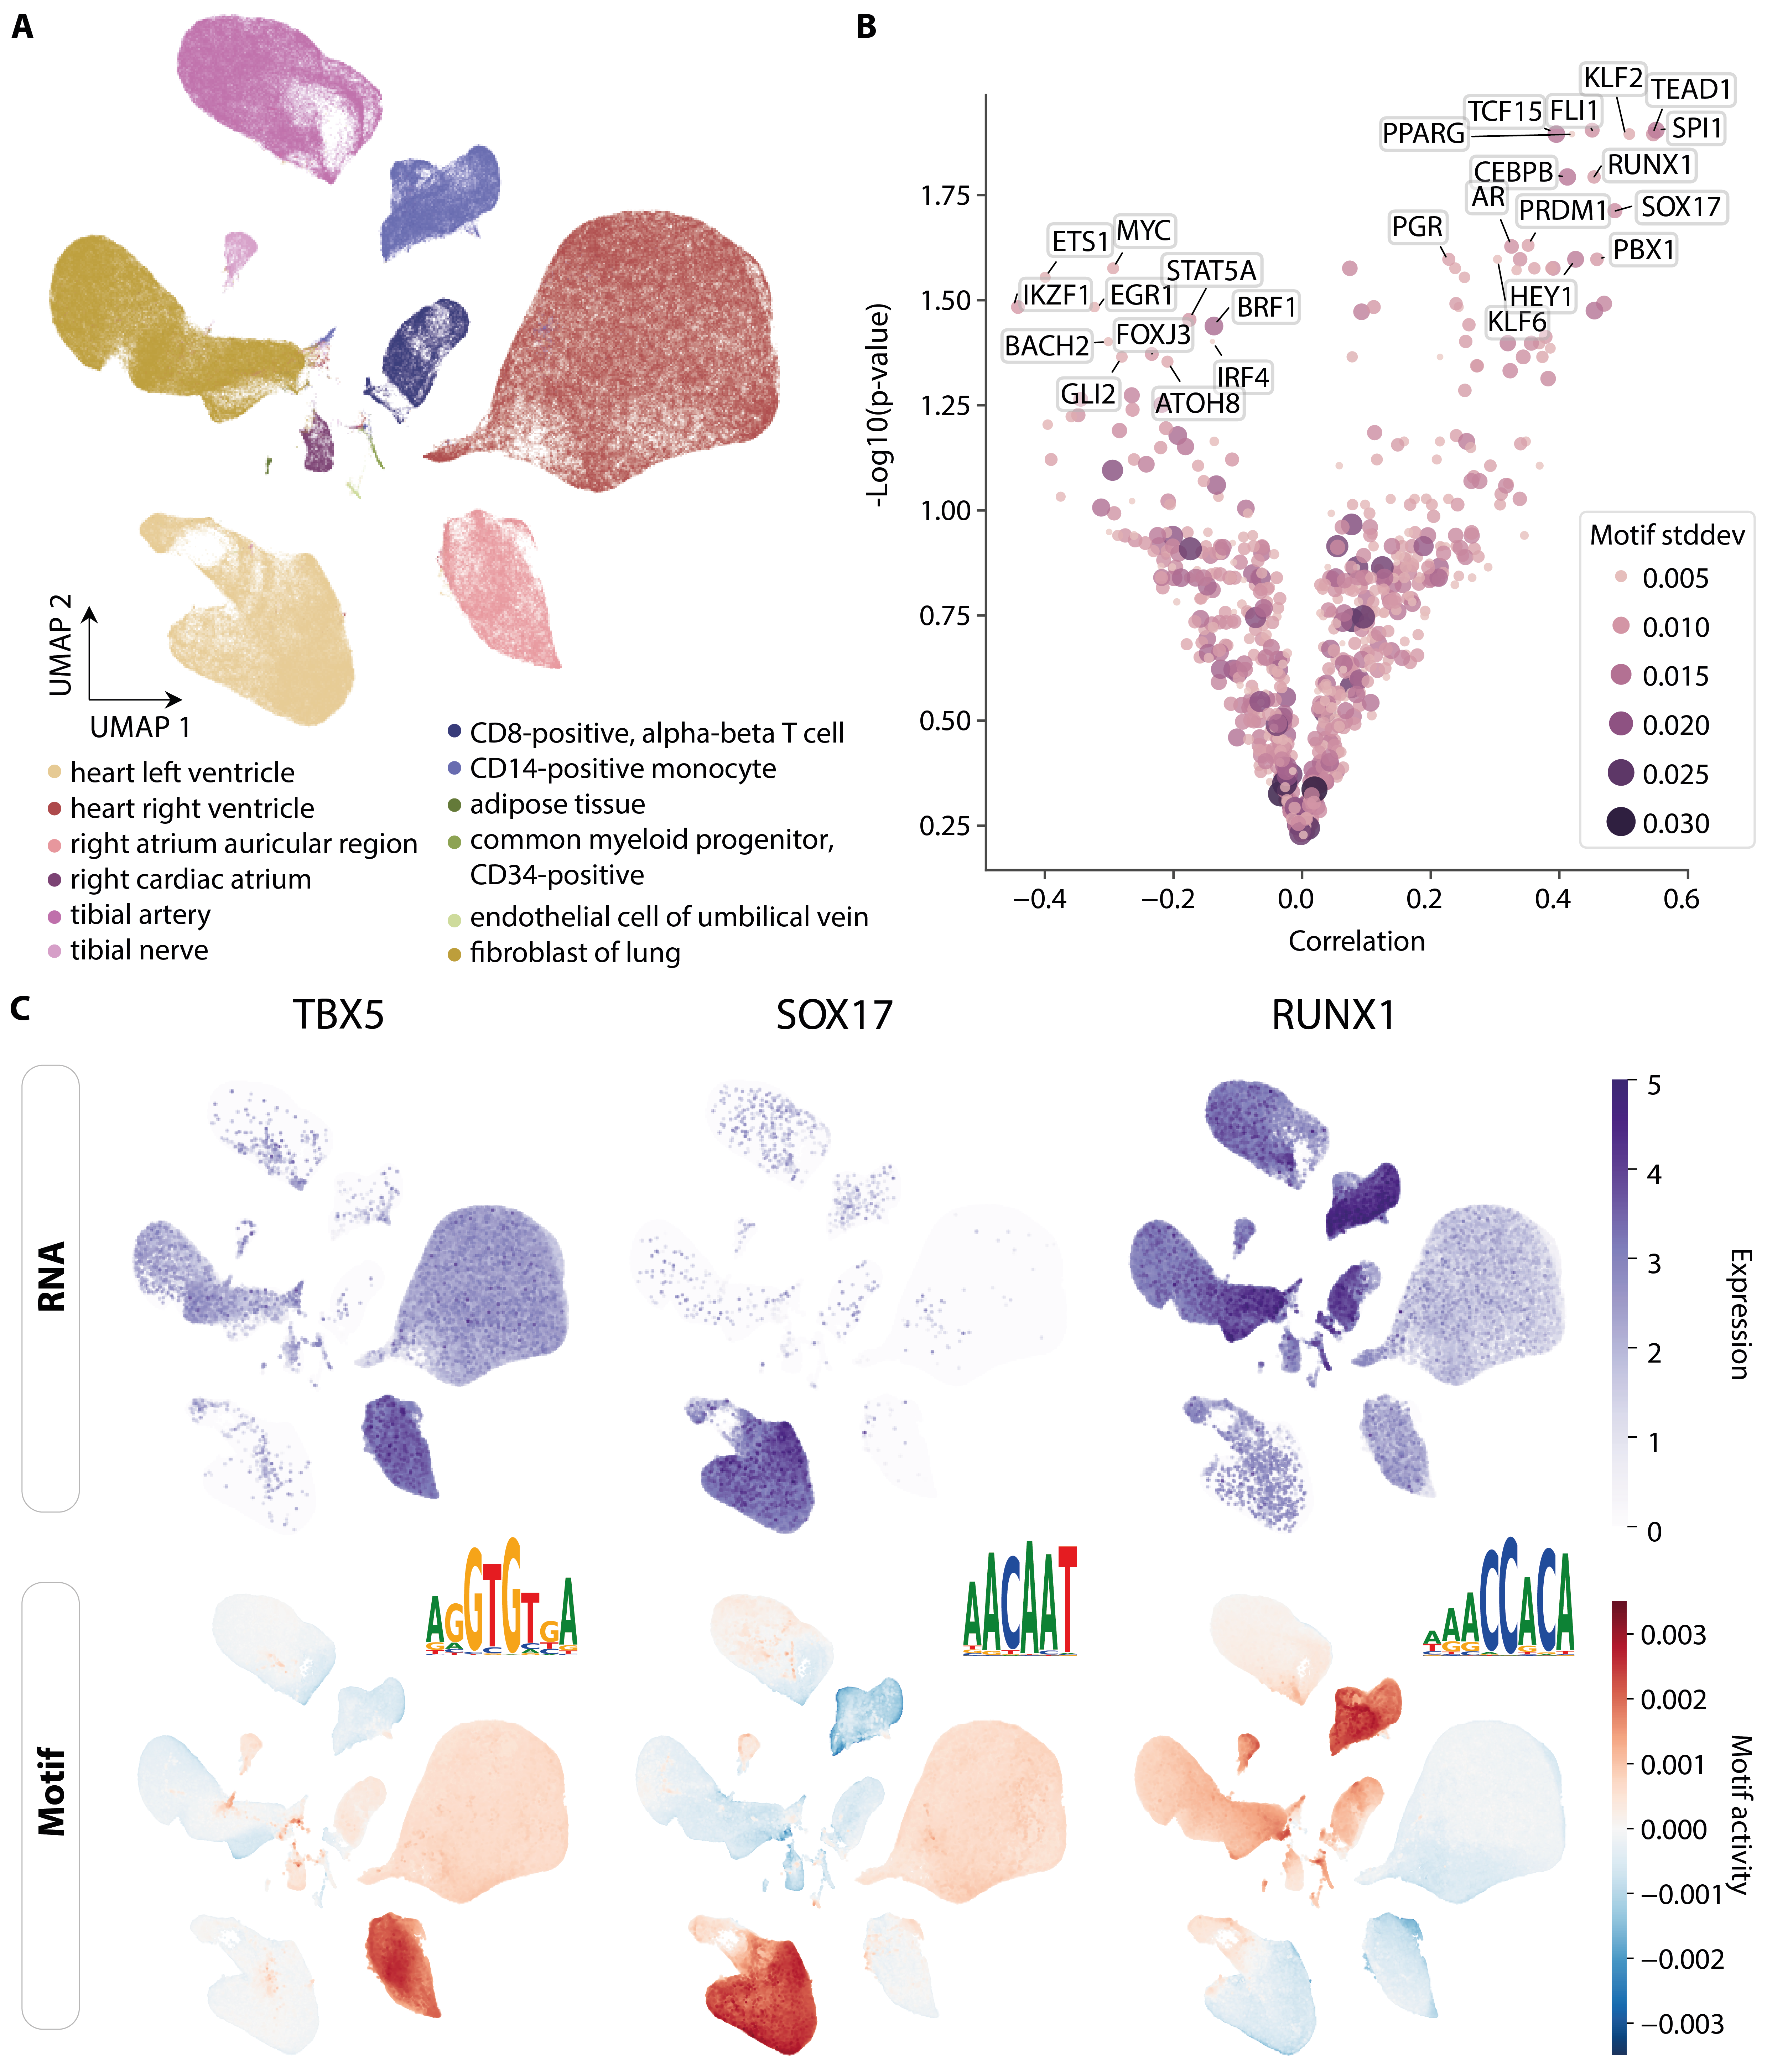
\includegraphics[width=0.75\linewidth]{ch.scepia/imgs/SCEPIA_allCells_v10_Myriad_Figure3.png}
    \caption{\textbf{Transcription factor activity in Human Heart Cell Atlas predicted by SCEPIA} \textbf{(A)} UMAP representation of all cells in the hHCA, based on UMAP coordinates provided by the original study\cite{Kanemaru2023}, with cluster annotation labels as predicted by SCEPIA. \textbf{(B)} Volcano plot of SCEPIA hits, where the x-axis is the correlation between motif and TF expression, and the y-axis is the log-likelihood of this correlation. The top 15 transcription factors are labeled, for putative positive regulators as well as putative repressors. Dot size and color labels are based on the motif score standard deviations. \textbf{(C)} Gene expression (top) and the corresponding predicted motif activity by SCEPIA (bottom), of three well-known markers: TBX5 (cardiomyocytes), SOX17 (endothelial cells), RUNX1 (blood cells). Sequence logos of the binding motifs are indicated, with the GimmeMotifs database identifiers (left to right): GM.5.0.T-box.0005, GM.5.0.Sox.0021, GM.5.0.Runt.0003. }
    \label{fig:scepia_hhca1}
\end{figure}

Following the initial annotation of cell types, we investigated the transcriptional regulators considered important by SCEPIA in these clusters. Among the top 15 hits, as ranked by their correlation coefficients, were several known markers for various cell types present in the atlas (Figure \ref{fig:scepia_hhca1}B). Examples include \textit{FLI1}, \textit{ETS1} and \textit{KLF2} for immune and endothelial cells \cite{Meadows2009,Zhao2018,BenDavid2022}, \textit{TBX5} for cardiomyocytes\cite{Steimle2017,Siatra2023}, \textit{HEY1} for atrial cardiomyocytes \cite{Kokubo2007}, and \textit{PPARG} for adipocytes \cite{Ma2018}. SCEPIA correctly predicted the motif activity of \textit{TBX5} in the cardiomyocyte clusters, which also aligned with its expression pattern (Figure \ref{fig:scepia_hhca1}C). Predicted motifs for \textit{SOX17} and \textit{RUNX1} exhibited variable motif activities, with expected higher activities in endothelial and lymphoid clusters, respectively (Figure \ref{fig:scepia_hhca1}C)\cite{Lee2014,Schachterle2017,Sood2017}. \textit{BACH2} is a known repressor and immune-regulating transcription factor and is also implicated in neural differentiation\cite{Hoshino2002,Liu2022}. \textit{BACH2} is most highly expressed in neural and lymphoid cells, where the motif activity (bZIP.0003) was decreased, and the reason for SCEPIA to identify this TF as a repressor (Figure \ref{fig:scepia_features1}A). However, the inferred motif activity of \textit{BACH2} was increased in the myeloid and endothelial cluster, contradicting its established role as a repressor in myeloid cells. \textit{BACH2} is known for its repressive regulatory functions in myeloid lineages \cite{ItohNakadai2014}, and was recently described for its activator role in B-lymphocytes\cite{Ochiai2022}. This duality, seemed to pose a challenge for correct inference of the activity for this factor in these cell types. This could be attributed to the absence of particular cellular subtypes in the H3K27ac reference, restricting the full capture of \textit{BACH2}'s complex transcriptional regulation in immune populations. To further confirm the regulatory role of \textit{BACH2} in this dataset, we checked the expression level for putative target genes, based on ChIP-seq (Fig. \ref{fig:scepia_features1}B). The compound expression level of 57 predicted \textit{BACH2} targets, showed patterns of expression similar to the motif activity as predicted by SCEPIA, and thereby for many clusters, the reversed of \textit{BACH2} expression itself. In summary, the \textit{BACH2} motif enrichment showed a similar pattern to the expression of its target genes, with a decreased motif activity in clusters exhibiting increased \textit{BACH2} expression. These findings underscore the difficulty of distinguishing some of the more complex regulatory roles of TFs. However, altogether SCEPIA mostly identified relevant regulators, as well as a well-known repressive regulator.

\begin{figure}
    \centering
    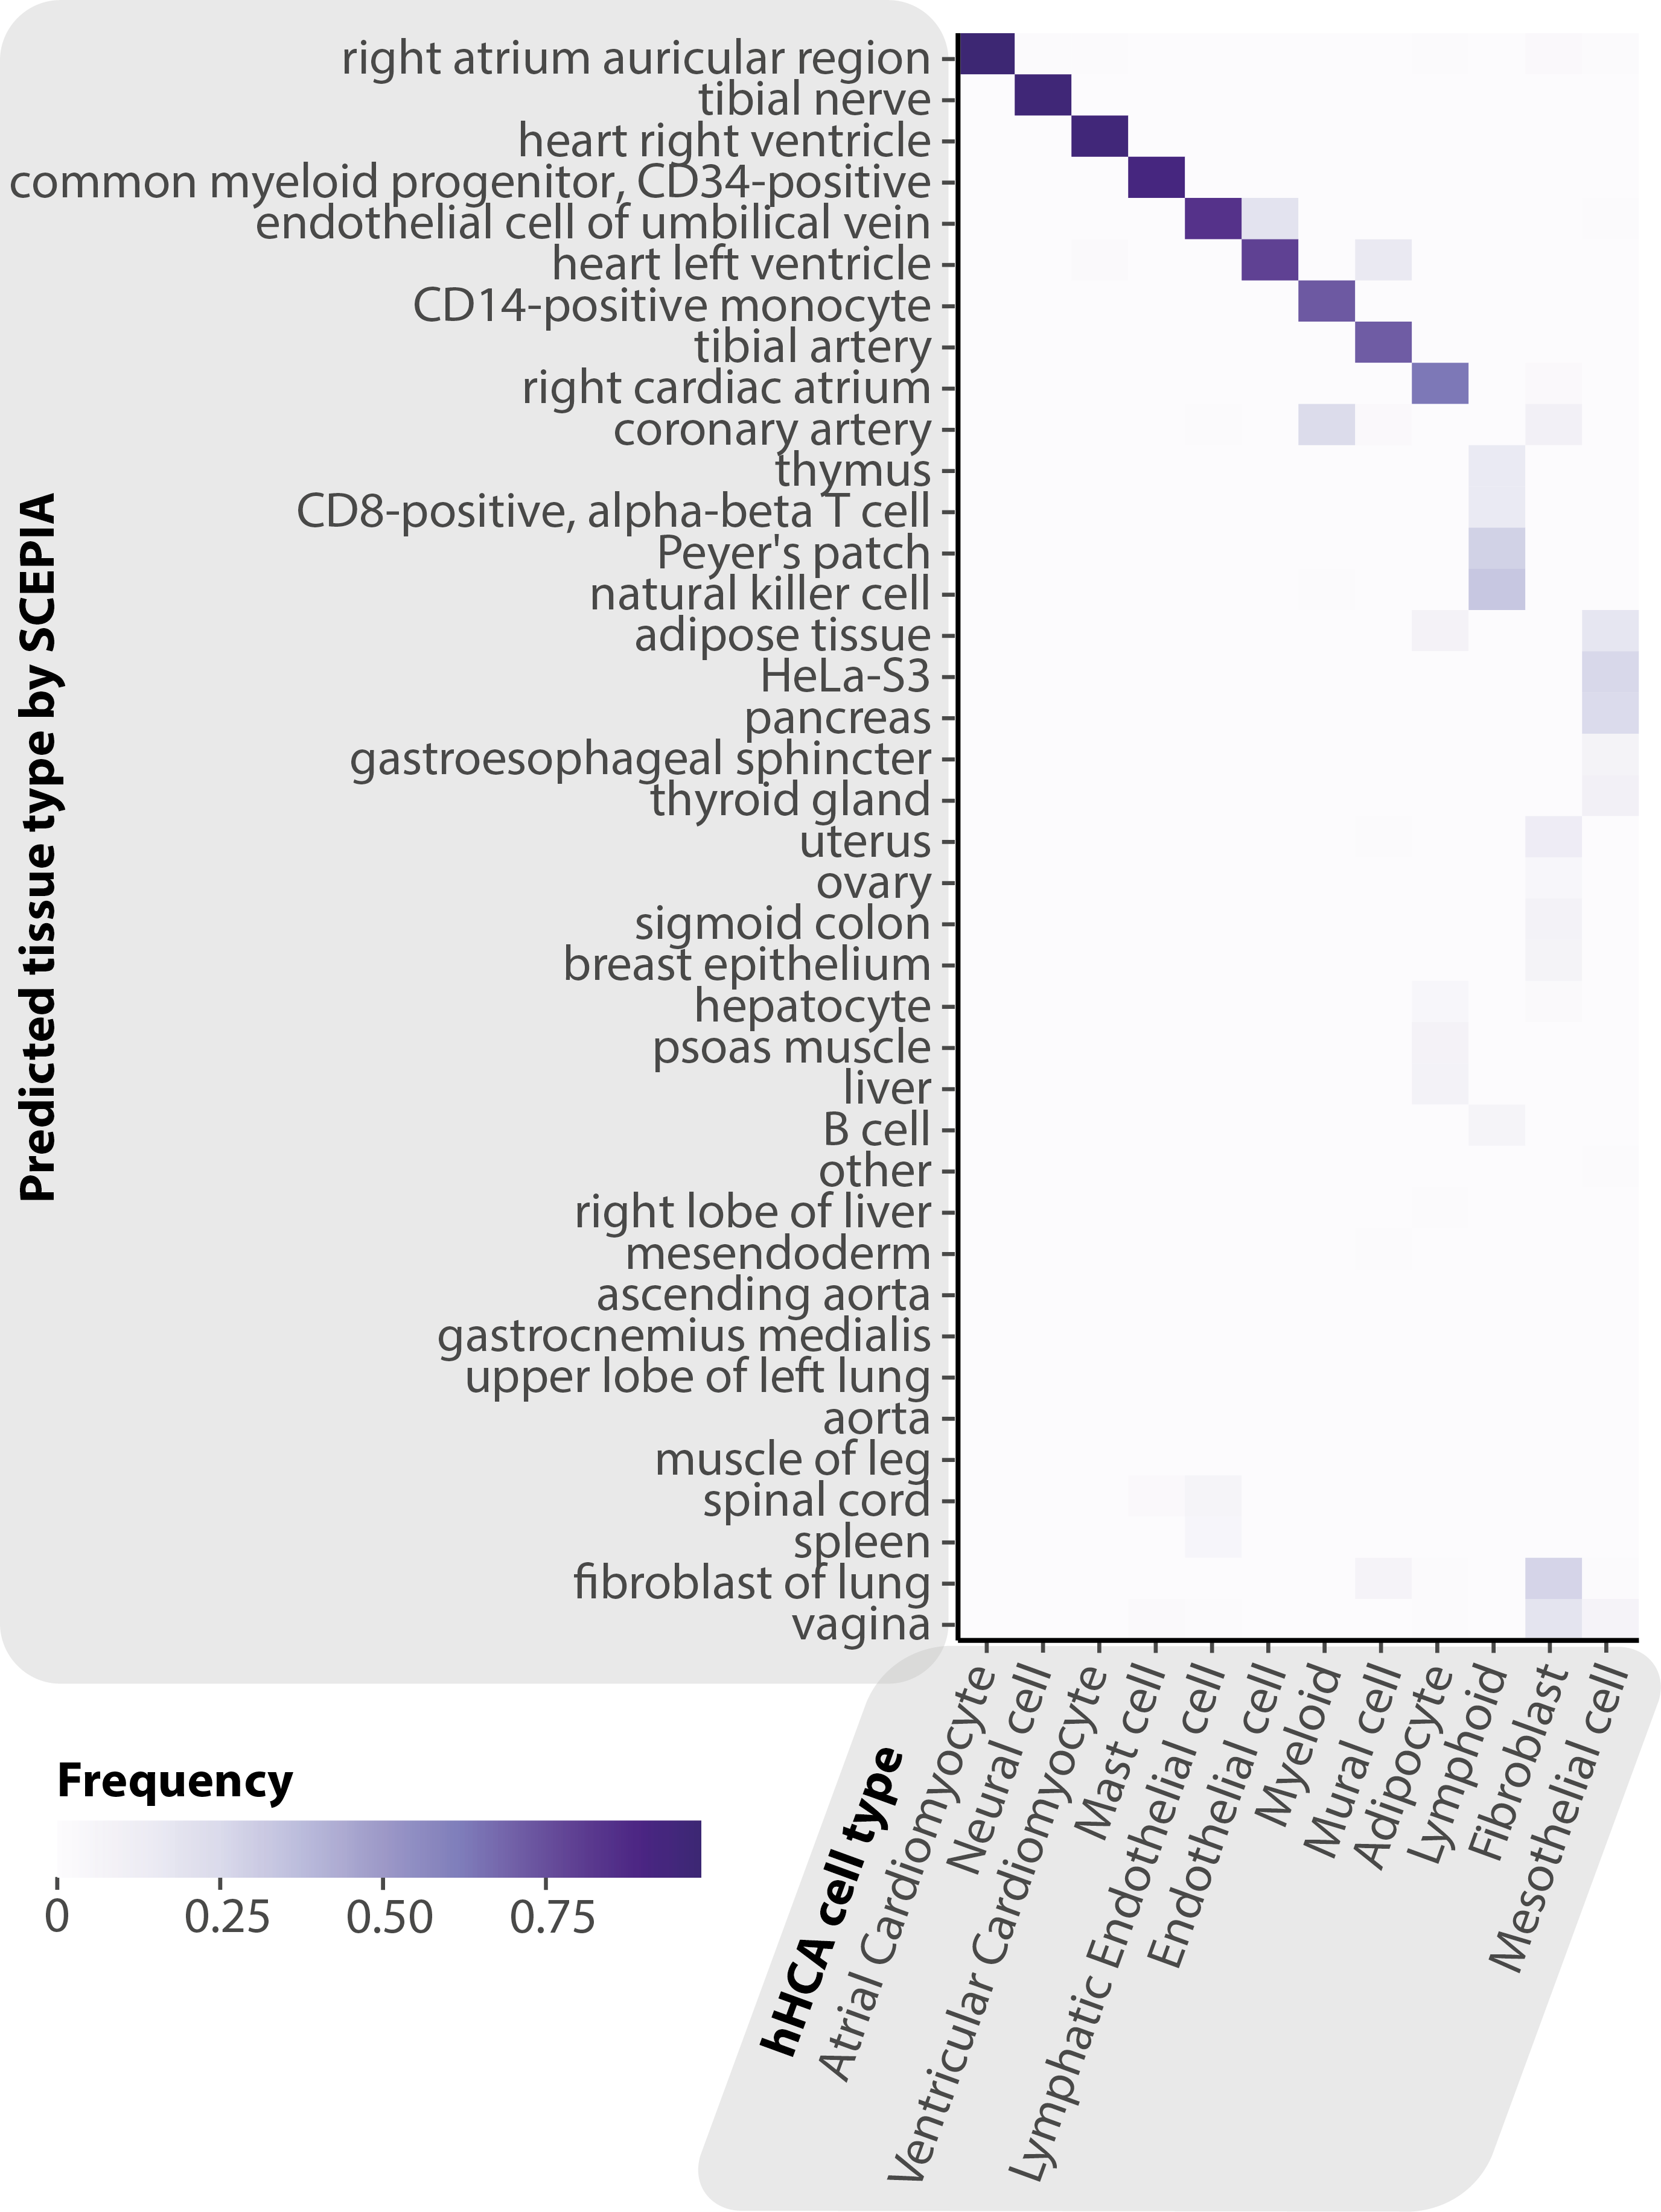
\includegraphics[width=0.75\linewidth]{ch.scepia/imgs/SCEPIA Annotation Heatmap All Cells 40deg Rotated Figure 4_noDend.png}
    \caption{\textbf{Evaluation of the SCEPIA cell type annotation} \textcolor{red}{Frequencies of cell type annotations as predicted per hHCA cluster by SCEPIAs annotation step. Cell annotations are used as weights per cell, allowing for combinations of cell or tissue types of the reference per cell that are be used in downstream analysis. To get an idea of the cell type annotation per cluster, the frequency of the highest matching reference cell or tissue type per cell are summed for each cluster and shown as proportions of cluster annotations in the heatmap.}}
    \label{fig:scepia_annohm}
\end{figure}

\subsection{Prioritization of cardiac regulators by SCEPIA improves with directed subsampling of abundant cell types}

For a subset of the hHCA, chromatin accessibility data (scATAC-seq) is available. For this data set, chromatin accessibility was measured in the same nucleus as the transcriptomic data. This offered an ideal use case for benchmarking SCEPIA. The multimodality allows for a comprehensive evaluation of transcriptional regulators identified by SCEPIA, as the predicted motif activity can be compared to the motif activity based on the scATAC-seq data. First, we ran motif analysis on the pseudobulk of the scATAC-seq clusters using GimmeMotifs Maelstrom\cite{Bruse_2018} (hereafter referred to as maelstrom analysis), to infer the cell type-specific motif activities. As mentioned, SCEPIA is tailored to infer enhancer activity from any epigenomic reference data, in this case, we used the ENCODE H3K27ac reference. Although the information on chromatin context between H3K27ac and ATAC-seq differs (active enhancers versus accessibility of chromatin, respectively), the motif analysis on the pseudobulk ATAC-seq served in this case as our closest approximation to a ground truth. 

To evaluate SCEPIA's performance in which gene expression is used as a proxy to retrieve information on chromatin accessibility, we set out to acquire a baseline of correlation coefficients for this type of analyses. Since we have the hHCA with transcriptomic information, as well as the chromatin accessibility of the same cell, we correlated TF expression with the binding motif activities of its clusters. The comparison is solely based on predicted motif-TF links from the GimmeMotifs database without any further prioritization and will thereby illustrate a baseline of coefficients that can be achieved comparing this type of multiomic data. To enable multiple runs in our comparisons and evaluate reproducibility, we divided the scRNA-seq data into seven random subsets, each consisting of 100K cells. Next, we correlated the motif activities computed with the maelstrom analysis with the expression levels of each binding TF across the cell types, and for each subset. This comparison yielded coefficients ranging from a r of -0.02 to 0.26 (Fig. \ref{fig:sc_benchmark} blue) and reflected the degree of similarity between TF expression levels and their motif activities measured in a single-cell multimodal setting.

To benchmark SCEPIA against these results, we compared the SCEPIA runs on each of these seven subsets to the maelstrom analysis. For all the significant SCEPIA hits (p-adj < 0.05), we averaged their inferred motif activities per cell type cluster. These averages were correlated to the activities for the same motifs from the maelstrom analysis. Interestingly, the mean coefficients per cell type in these correlations were consistently higher than those found in the baseline comparison, except for the mesothelial and mural cell cluster (Fig. \ref{fig:sc_benchmark} orange, Table \ref{tab:significance_scbenchmark}). However, these scores exhibited substantial differences across the cell types, with a median r ranging from 0.14 for the mesothelial to 0.58 for the myeloid cluster (Table \ref{tab:significance_scbenchmark}).

As we observed variations in the performance across the cell types, with some scoring lower (e.g. cardiomyocyte clusters, fibroblasts and endothelial cells, with a median r < 0.4), than others (myeloid and mast cell clusters, median r > 0.4), we implemented a step of geometric sketching. Geometric sketching is a method that subsamples the cells in the dataset while preserving the inherent heterogeneity, or geometry, of the dataset \cite{Hie2019}. Since a geometric sketch will lead to a more equal representation of the different cell types across the dataset, including rare cell types, we included this subsampling step during the pre-processing of the data and preceding the SCEPIA run on each of the seven subsets (see Methods). This significantly improved the correlation coefficients with the maelstrom results for both cardiomyocyte and endothelial clusters, as well as the myeloid cluster (Fig. \ref{fig:sc_benchmark} green, Table \ref{tab:significance_scbenchmark}). The neural and adipocyte, mural and mesothelial cell-clusters displayed more variability in their coefficients, with some obtaining equal or worse coefficients after the addition of the geosketching. While the geometric sketch could not fully alleviate the relatively low performance of SCEPIA for certain cell types, incorporating this step significantly improved the performance for five out of the twelve cell clusters in this specific benchmark. 

\begin{figure}
    \centering
    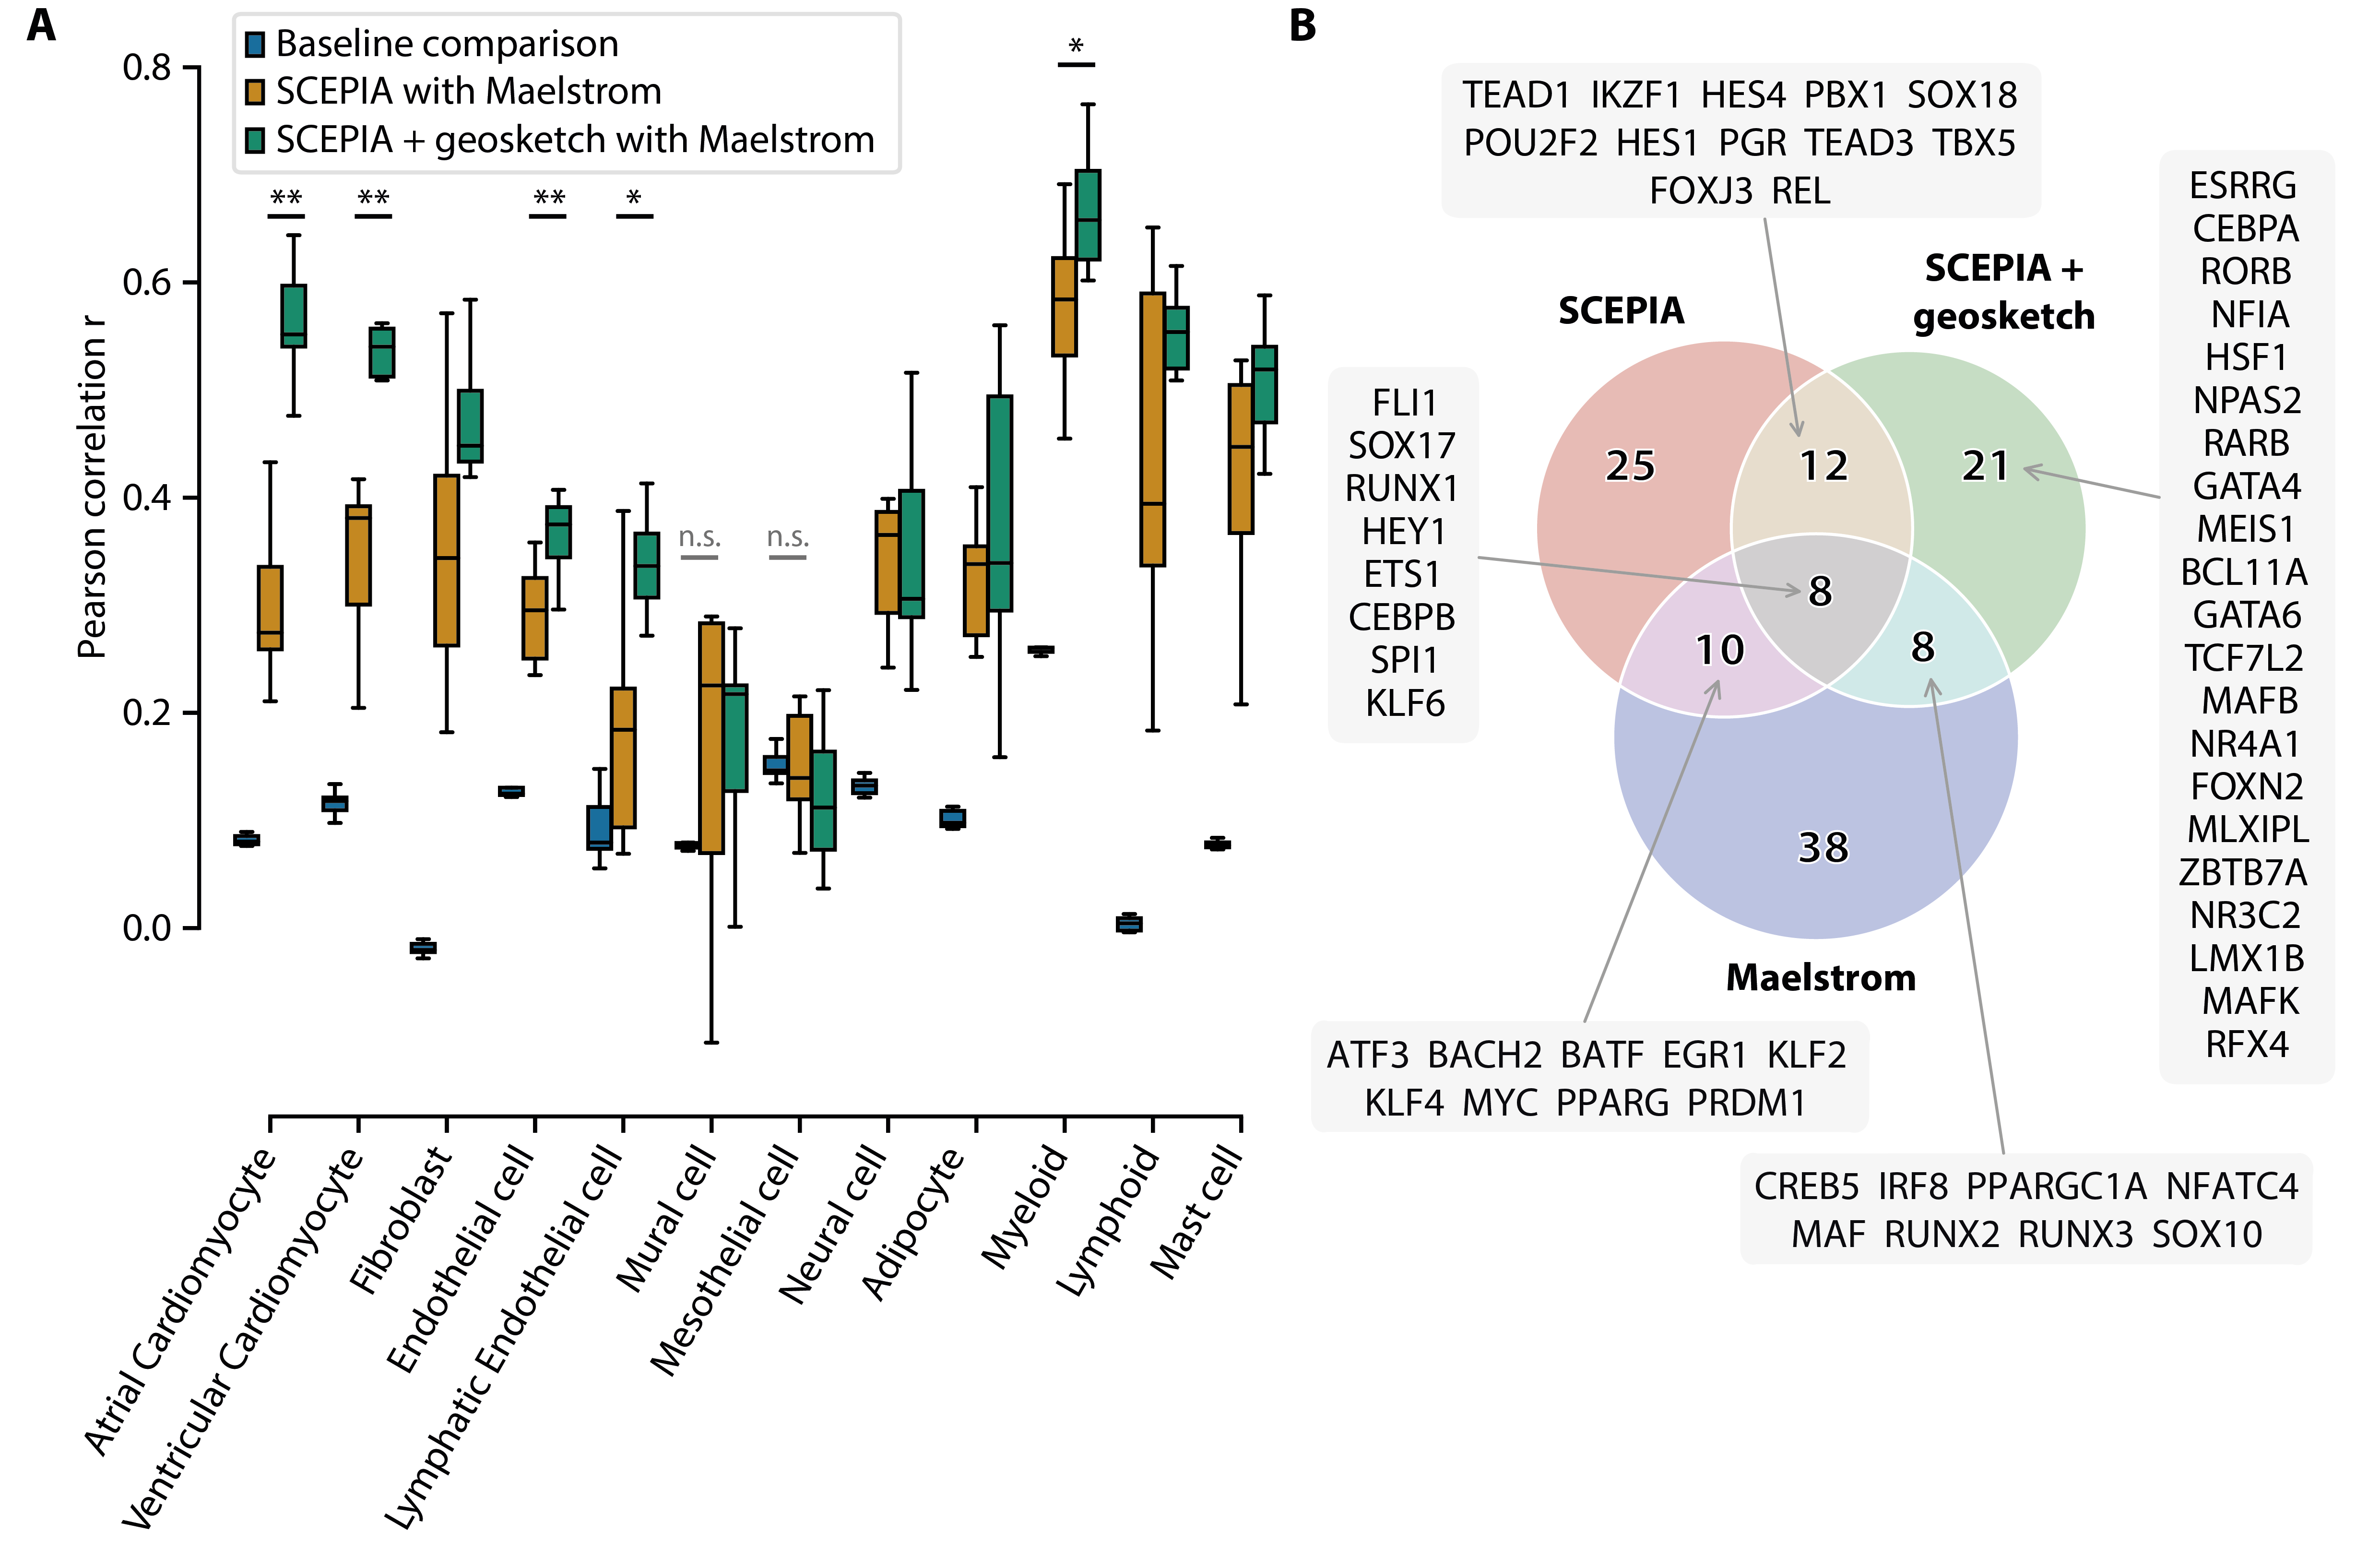
\includegraphics[width=0.75\linewidth]{ch.scepia/imgs/OverlappingHitsBetweenSCEPIAGEOANDMAELSTROM_BlackMyriad_onlySign_baselineNS_v11_Figure4.png}
    \caption{\textbf{Benchmarking SCEPIA results between repeated runs and with a geometric sketch of the data} (\textbf{A}) Correlations between motif activity computed in pseudobulk ATAC-seq fraction (maelstrom analysis) and expression values of the corresponding TFs from each of the seven 100K cells scRNA-seq subsets (blue; Baseline correlations). In orange the motif activities of significant (p-adjusted < 0.05) SCEPIA hits from each of the seven 100K subset analyses, were correlated with the matched motif activities computed with the maelstrom analysis (SCEPIA with Maelstrom). Green represents the correlation coefficients of the comparisons with maelstrom motif activities, for the seven 100K subset runs with SCEPIA with prior pre-processing with geometrical sketch subsampling of each of the seven 100K cells subsets (SCEPIA+geosketch with Maelstrom). Significance of differences between conditions was calculated with the one-sided Wilcoxon signed-rank test. Only non-significant results are indicated for the baseline versus SCEPIA comparison in grey, and only significant results indicated for the SCEPIA versus SCEPIA+geosketch comparisons (all p-values can be found in Table \ref{tab:significance_scbenchmark}).  **: p-value <= 0.01, *: p-value <= 0.05, n.s.: non-significant. (\textbf{B}) Venn diagram presenting overlaps and differences between the SCEPIA runs on the full dataset (700K cells of the hHCA), the SCEPIA run with geosketch subsampling of the full dataset (subsampling 700K to 20K cells) and the maelstrom analysis on the pseudobulk of the scATAC-seq data of the hHCA. hHCA = human Heart Cell Atlas.}
    \label{fig:sc_benchmark}
\end{figure}

\subsection{SCEPIA identifies additional cardiac regulators compared to motif analysis in ATAC-seq} 

To validate our approach in selecting regulatory factors based on motif activity and TF expression patterns, we compared the outcomes of SCEPIA with a selection based on motif activity alone. Given the improved performance of SCEPIA across various cell types with the inclusion of a step of geosketching, we further examined its efficacy by downsizing the full dataset to a geosketch of 20K cells and reran SCEPIA (Fig. \ref{fig:geoscepia_results}). We then explored biological differences between the methods.

Of the 49 total hits, the geosketched SCEPIA run yielded 20 overlapping hits with the full dataset run and a partial overlap with TFs linked to maelstrom motif hits (16 hits; Figure \ref{fig:sc_benchmark}B). Common hits, such as \textit{FLI1} and \textit{SOX17}, implicated in cardiac cells, as well as \textit{HEY1} (cardiac progenitor marker) and \textit{ETS1} (lymphoid marker), reaffirmed SCEPIAs consistency. The maelstrom analysis pointed to variable motif activity for a BACH2-binding motif and indicated higher activity in the fibroblast, endothelial and mesothelial clusters. The first SCEPIA run inferred increased motif activity for \textit{BACH2} in these same clusters, with additional high levels in the myeloid and mural cells (Figure \ref{fig:scepia_features1}A). However,  differences also emerged between the runs. \textit{GATA4} and \textit{GATA6} for example, vital for cardiac (mesoderm) development and inferred with increased motif activities in the cardiomyocyte clusters, were exclusively found in the run on the data preprocessed with geosketch (Figure \ref{fig:scepia_features1}C) \cite{Morrisey1996,Song2022}. Notably, \textit{GATA1} was only identified in the non-geosketched run, showing specific expression and increased motif activity in mast cells (Figure \ref{fig:scepia_features1}D), a cell type-specificity confirmed in literature \cite{Migliaccio2003,Gao2015}. \textit{RUNX1} was consistent, while \textit{RUNX2} and \textit{RUNX3} were additionally identified in the geosketch run, all linked by SCEPIA to the same motif (Runt.0003). The motif activity changed to be more restricted to immune cells in the geosketch run, whilst in the run without geosketch this motif activity was additionally inferred across, for instance, the mural, neural and fibroblast cells (Figure \ref{fig:scepia_features1}E, \ref{fig:scepia_hhca1}C).

The overlapping hits between geosketch SCEPIA and the maelstrom analysis revealed specific points of interest. Of the \textit{SOX} gene family, \textit{SOX17} and \textit{SOX18} emerged in the initial SCEPIA run, associated with motifs that exhibited similar activities across the clusters. The geosketch SCEPIA analysis additionally revealed \textit{SOX10} in the neural and, to a lesser extent, endothelial cells (Figure \ref{fig:scepia_annotation1}F). Similarily, maelstrom identified two \textit{SOX10} motifs ranking among the top three in the neural cluster (specifically Sox.0018 and Sox.007; Figure \ref{fig:scepia_maelstromhm}). This cluster was highlighted in the original paper for its pan-glial marker expression. Therefore these \textit{SOX10} results are in line with its significance in neural crest development and pivotal role in differentiation to neuronal or glial cells \cite{Lai2021}. Furthermore, SCEPIA not only confirmed a similar motif specificity for \textit{SOX10} in this dataset, but also identified a motif sequence which corresponds to a subset of the motifs inferred by maelstrom (Figure \ref{fig:scepia_features1}G). Differences included \textit{IKZF1}, identified by SCEPIA with an inferred activity in almost all clusters, with only a specific depletion of signal in the immune clusters (Fig. \ref{fig:scepia_features2}B, D), aligning with its dual repressor and activator role in immune cells \cite{Marke2018}. Other examples were \textit{TBX5} and \textit{MEIS1}, both well-known cardiac mesoderm markers, alongside \textit{ESRRG}. Binding motifs for these factors were inferred with an activity across multiple, if not all, clusters in the dataset. Only by additionally considering the expression levels of the binding TFs, a specificity became apparent (example of \textit{ESRRG} in Fig. \ref{fig:scepia_features2}A, C). Conversely, there were also hits in Maelstrom, that were not identified in any of the SCEPIA runs. A notable discrepancy involved the \textit{MEF2} transcription factor family. Maelstrom analysis showed motif enrichment in cardiomyocytes and mural cell clusters, however, the expression levels of \textit{MEF2A-D} were consistent across the majority of cell types (Fig. \ref{fig:scepia_features2}E) and showed low correlations with their inferred motif activities (Tables \ref{tab:corrtable_SCEPIA} and \ref{tab:corrtable_GeoSCEPIA}), which could explain the absence in SCEPIAs hits. These findings suggest that SCEPIA is better suited in identifying factors with ubiquitous motif activities, because of the inclusion of expression level information in selecting the factors. Conversely, if the expression of the factor is not highly variable or not well (anti-)correlated with the predicted motif activities, SCEPIA will overlook these factors, even if the binding motifs were inferred with variable activities over the cell types.

Several mesothelial regulators mentioned by the authors of the hHCA, \textit{WT1} and \textit{BCN1}, or other epicardial marker genes (\textit{TBX18} and \textit{TCF21}) were not found in our maelstrom analysis of the hHCA scATAC-seq data \cite{Wu2013}. This could explain the difficulty in predicting the appropriate regulators for this and similarly small clusters, which are lost by performing the analysis on this whole dataset at once. This could also explain why some of the cell types are not performing well compared to more abundant clusters in the dataset. Looking at the cluster sizes in the scATAC-seq data: XX cells were found for the mural and mesothelial cluster, respectively.

\section{Discussion}

In this study, we present SCEPIA, a novel computational method for inferring transcription factor motif activities using single-cell transcriptomic data in combination with a reference H3K27ac collection. SCEPIA successfully identifies established key regulators in various cardiac cell types, including endothelial cells (\textit{FLI1}), cardiomyocytes (\textit{TBX5}, \textit{HEY1}), adipocytes (\textit{PPARG}), and immune cells (\textit{RUNX1}), in addition to recognizing the suppressor \textit{BACH2}. This method stands out by leveraging pre-existing bulk epigenomic data, thus augmenting single-cell transcriptomics datasets and creating a multimodal resource for the identification of transcription regulators.

SCEPIA matches cells to a combination of known H3K27ac signatures, thereby establishing new H3K27ac identities that are not explicitly defined in the reference. In the case of cardiac endothelial cells and adipocytes, which were both missing from the reference, this approach has demonstrated that it can identify appropriate key TFs (\textit{e.g.} \textit{FLI1} and \textit{PPARG}). However, we faced challenges with the identification of key TFs for other cell types that were not in the reference, such as mesothelial or mural cells. This difficulty likely arises from two main issues: the lack of closely related cell types in the reference dataset (for example, epicardial cells) and the low number of these cells in the cardiac tissue samples we studied. One solution for this could potentially be found in expanding on the current ChIP-seq reference in SCEPIA. Expanding the provided references with other epigenomic collections, either generated by the researcher themselves or using readily available and vast collections (e.g. SRA) could greatly enrich SCEPIA's reference database and potentially improve its accuracy and applicability, also for more rare subtypes. Alternatively, one could subset the data even further, to only include a subset of specific cell types. 

The transcription factor \textit{MEF2C} plays a crucial role in chromatin remodeling which increases DNA accessibility in cardiomyocytes\cite{Stone2019,Ieda2010,Desjardins2016} and during neural development\cite{Li2008}. Despite its important role, SCEPIA did not identify \textit{MEF2C} or other members of the \textit{MEF2} family, as key cardiac regulators. However, in our comparison based on single-cell DNA accessibility alone, their motif was flagged for its differential inferred activity. Even though we observed a variable gene expression of \textit{MEF2C} across different cell types, there was a poor match between the gene expression levels and predicted motif activity. This exemplifies the complex nature of the role of \textit{MEF2C} in regulating genes during heart development. \textit{MEF2C} is known to produce several isoforms that regulate different genes\cite{Zhu2004}. Additionally, \textit{MEF2} factors often form hetero- or homodimers to more precisely regulate their target genes \cite{Desjardins2016,Black1998}. The complexity of the \textit{MEF2} gene regulatory function demonstrates the drawback of transcriptomic-based regulator inference methods, including SCEPIA. These methods cannot account for post-transcriptional modifications, and as such cannot fully capture the regulatory roles of transcription factors like for instance, \textit{MEF2C}.

Establishing an accurate baseline and ground truth presents a significant challenge in our study, particularly when it comes to benchmarking the results of SCEPIA. For the single-cell comparisons, our ground truth is calculated on regression coefficients based on a measure of DNA accessibility. However, SCEPIA uses a different reference, based on H3K27ac, a marker for active cis-regulatory regions. Whilst DNA accessibility and H3K27ac generally coincide, these two assays measure distinct aspects of chromatin context and gene regulation. For instance, our SCEPIA analysis identified nuclear receptor motifs, such as \textit{TBX5} and \textit{GATA4}, using the H3K27ac reference. These motifs were not detected based on our analysis of scATAC-seq data. This discrepancy can be attributed to the nature of these transcription factors: \textit{TBX5} and \textit{GATA4} need co-factors to bind the chromatin and activate their targets, and are not able to bind previously inaccessible regions\cite{Stone2019}. Therefore, ideally, both the reference database and the ground truth are based on the same assay. Additionally, the motif activities based on DNA accessibility in SCEPIA are inferred by the ensemble computational method GimmeMotifs Maelstrom\cite{Bruse_2018}. As a consequence, the ground truth of this study is based on a computational analysis rather than an experimentally validated ground truth. Lastly, by only correlating the activities for the exact same motifs between the maelstrom analysis and the SCEPIA outcomes, we underestimate SCEPIAs performance. The activity of a TF will be shared over all of its potential binding motifs in the regressions performed, and only the motif activity that correlates best with the TF's expression, will in the end be linked to the TF. Meaning, there is no guarantee, or need, for these motifs to be exactly the same in both analyses.

We foresee several ways to improve the current implementation of SCEPIA. First,the appropriate selection of highly variable genes and relevant cells can be improved. Currently, SCEPIA selects the top 2,000 genes based on dispersion-normalized gene expression, which may inadvertently bias the analysis towards overrepresented cell types. Potentially more sophisticated approaches could be used, such as comparing the highly variable genes between clusters, performing geometry-preserving sampling (geosketch)\cite{Hie2019}, or selecting genes based on selectively detected or undetected expression in a particular cell neighbourhood (SEMITONES)\cite{Vlot2022}. Cell sampling methods that represent all distinct cell types, such as geosketch, have as an added benefit that the TF-motif significance calculation will be improved. Currently, TF-motif significance is calculated with a permutation test of the correlation between TF and motif. The presence of large groups of similar cells influence this calculation, therefore a more representative subsampling of the data could be beneficial. Second, SCEPIA could be improved by incorporating additional genomic assays. Given the similarities between H3K27ac and ATAC-seq data, integrating an extensive ATAC-seq collection seems promising. SCEPIA already includes pre-built references from diverse sources, such as scATAC-seq datasets of fetal human cell types\cite{Domcke2020} and various adult mouse tissues\cite{Cusanovich2018}. Third,the permutation test on the correlation coefficient between TF and motif activity can be refined. The relationship between TF gene expression and its motif activity is often unclear. Instead, a more informative relationship can be found between motif activity and the gene expression of downstream genes. Given that SCEPIA includes a comprehensive reference of cis-regulatory regions, these regions can be associated to their nearest gene, although this approach has its limitations\cite{Fulco_2019}. By establishing this association, we can link motif activities directly with specific genes, thereby basing the significance test on a more direct and relevant relationship. Moreover, combining these relationships with the expression of the TF itself, provides a clearer understanding of the functional impact of TFs within regulatory networks.

% Conclusion
Single-cell omics datasets provide a detailed view of transcription regulation unique to each cell type, enabling the exploration of lesser-known and more challenging-to-obtain populations within tissues. Given that heart and vascular diseases are among the leading causes of death worldwide\cite{Tsao2023}, it is crucial to better understand epigenomic (dis)regulation at a cellular level. Our study introduces SCEPIA, a powerful computational tool designed to enrich single-cell transcriptomic data with transcription factor motif activity. This enhancement facilitates the precise identification of regulators specific to different cell types. The capability of SCEPIA to integrate detailed transcription factor information into single-cell transcriptomics paves the way for a more comprehensive understanding of how transcription is regulated in various cell types.

\section{Methods}

\subsection{Overview of public data}

\subsubsection{Sequencing data}

Full sample tables can be obtained from \url{https://zenodo.org/doi/10.5281/zenodo.10457767}.

\subsubsection{Cis-regulatory regions}

We used a collection of cis-regulatory regions, based on all human transcription factor ChIP-seq peaks from ReMap 2018\cite{Chneby2017} (\url{http://remap.univ-amu.fr/storage/remap2018/hg38/MACS/remap2018_all_macs2_hg38_v1_2.bed.gz}), as described previously\cite{Xu_2020}. This collection of cis-regulatory regions is available at Zenodo (\url{https://zenodo.org/records/4066424}).

\subsubsection{Human heart cell atlas}

The human heart cell atlas transcriptomes covered 704,296 cells and nuclei and was obtained as a matrix with log-normalized counts\cite{HHCA_RNA_gene_matrix}. Part of the atlas was sampled with 10X Multiome, and thereby consisting of scATAC-seq assay covering 144,762 nuclei, which was downloaded as a raw peak count matrix\cite{HHCA_ATAC_peak_matrix}.

\subsection{RNA-seq processing}

Preprocessing of RNA-seq was done automatically by seq2science v1.0.3 \cite{seq2science} using the RNA-seq workflow. Public samples were downloaded from the Sequence Read Archive \cite{Leinonen2010} with the help of the NCBI e-utilities and pysradb\cite{Choudhary2019}. Genome assembly GRCh38.p13 was downloaded with genomepy 0.16.1 \cite{Frlich2023}. Paired-end reads were trimmed with fastp v0.23.2 \cite{Chen2018} with default options. Reads were aligned with STAR v2.7.10b \cite{Dobin2012} with default options. Afterwards, duplicate reads were marked with Picard MarkDuplicates v3.0.0 \cite{picard}. BAM files were converted to CRAM format with samtools v1.16 \cite{Danecek2021}. Read counting and summarizing to gene level was performed on filtered BAM files using HTSeq-count v2.0.2 \cite{Anders2014}. TPM-normalized gene counts were generated using genomepy based on longest transcript lengths.

\subsection{H3K27ac ChIP-seq processing}

We downloaded 327 H3K27ac aligned samples from the ENCODE data portal\cite{encode_dcc}, spread over 121 cell types. For each sample, the coverage over the remap peaks was computed by the GimmeMotifs coverage\_table command\cite{Bruse_2018}. The values between samples was quantile normalized\cite{qnorm}, and consequently log2(x+1) normalized.

\subsection{Regulatory potential}\label{section:regpotential}

The cell type-specific regulatory potential P of gene $g$ is calculated similar to\cite{Wang2016}:
\begin{equation*}
    P_g = \sum_k w_{k}s_{k,g}
\end{equation*}
where $w_k$ is the weight at position $k$, and $s_{k,g}$ is the h3k27ac signal at position $k$ for gene $g$.

\noindent
The weight $w_k$ is calculated identically to the method ANANSE\cite{Xu_2020}:
\begin{equation*}
    w_k = \begin{cases}
        1, & \text{if } k \in (0\,\text{kb},\ 5\,\text{kb}] \\
        \frac{2e^{-\mu|k-t_g|}}{1+e^{-\mu|k-t_g|}}, & \text{if } k \in (5\,\text{kb},\ 100\,\text{kb}]
    \end{cases}
\end{equation*}
where parameter $t_g$ is the genomic position of the TSS of gene $g$, and $\mu$ determines the decay rate as a function of distance from the TSS, set such that an enhancer 10 kb from the TSS contributes one-half of an enhancer within 5 kb from TSS. $t_g$ is the distance from the TSS.

\subsection{Regulatory motif analysis and motif and transcription factor activity}

In the regulatory potential benchmark (Fig. \ref{fig:bulk_comparison}B) and in SCEPIA we use the motif activity as a measure of motif and transcription factor importance. The motif activity\cite{FANTOM2009, Balwierz2014} is calculated using Bayesian ridge regression implemented in gimmemotifs\cite{Bruse_2018}, with the motif log-odds scores as features and the H3K27ac signal as predictor variable. In short, for each cis-regulatory region in the input we compute the motif log-odds score for each motif in the gimmemotifs database (gimme.vertebrate.v5.0). This motif databases contains a non-redundant collection of vertebrate transcription factor motifs\cite{Bruse_2018}. We assume that the H3K27ac signal in each enhancer, expressed as log2(nr of reads + 1), is the sum of all motif log-odds scores multiplied by their respective motif weights. We then estimated these motif weights using Bayesian ridge regression, where the regularization parameter ($\lambda$) was determined through 5-fold cross-validation. These motif weights, the feature coefficients from the fitted regression model, are used as a measure of motif importance, the motif activity. This measure can then be used as transcription factor activity based on the TFs that are predicted to bind to the motif.

\subsection{Benchmark of regulatory potential-based cell type and motif assignment.}

To assess the performance of the regulatory potential-based approach compared to the actual H3K27ac signal, we conducted a systematic analysis. Our approach involved data subsampling and calculating correlation coefficients to evaluate the relationship between the ground truth and the regulatory potential-based approach. Specifically, this analysis used two data sources: the bulk H3K27ac reference database encompassing 121 tissues from ENCODE and 1,268,775 REMAP peaks, as well as the RNA-seq database featuring 96 tissues from ENCODE.

To establish a ground truth for comparison, we calculated the motif activity using the top 25,000 enhancers with the highest coefficient of variation with GimmeMotifs version 0.18.0\cite{Bruse_2018}. We selected random subsets of five tissues from tissues shared between the RNA-seq database and the H3K27ac reference database, and calculated the Pearson correlation coefficients between the estimated motif activity and the ground truth motif activity for each tissue in each comparison.

As our baseline approach to estimating motif scores, we consider the transcripts per million (TPM) of a transcription factor directly as the motif score. When multiple transcription factors are associated with a single motif, we use their average expression.

In the regulatory potential-based approach, we exclude the five ground truth tissues from the reference database. We then convert the H3K27ac signal from the reference database into regulatory potential and subsequently perform regression analysis against the TPM values. This results in a (5 x nr cell types) table of regression weights. We select the top 50 tissues with the highest absolute regression weights and identify the top 10,000 differential enhancers between them. We then conduct a motif scan similar to the one performed for the ground truth, regressing the H3K27ac signal with the motif scores in these enhancers. Finally, the motif scores for our original five tissues are calculated by taking the dot product of the motif scores in the top 50 tissues and the tissue weights.

\textbf{To assess the impact of using only the top 10,000 peaks for the regulatory-based approach while retaining the top 25,000 peaks for the ground truth, we also compute motif scores based on the top 10,000 differential enhancers (again selected based on the coefficient of variation).}

This entire process was repeated one hundred times to generate a distribution of correlation coefficients, providing an estimate of the performance of each approach.

\subsection{Detailed description of the implementation of SCEPIA}

The single-cell regulatory-based approach (SCEPIA) is similar to the bulk approach. However, due to the  increase in data, some steps need to be altered from a computational resource point of view. In addition, the fact that a single-cell dataset usually consists of multiple related cell types, with a more fluent gradient in gene expression and thus motif scores, makes it so that this information can be used to infer the significance of differential transcription factors based on motif scores and gene expression data.

\noindent
Required input:

\begin{itemize}
	\item Reference database matrix of peak intensities (D) with dimensions (peaks x cell types). SCEPIA comes with multiple extensive reference databases, and the user does not need to provide these themselves. These reference databases can be extended, however.
    \begin{itemize}
        \item The default human reference is based on REMAP 2018\cite{Chneby2017}, and consists of 1,268,775 putative enhancers. It contains 121 ENCODE\cite{encode_dcc} cell types. The number of reads in these enhancers per cell line was log2(x + 1) transformed, and quantile normalized\cite{qnorm} to enforce the same distribution.
        \item The default reference database is based on H3K27ac signal, but this can be any chromatin mark associated with regulatory activity, for example, ATAC-seq.
    \end{itemize}
	\item Single-cell RNA-seq dataset S with dimensions (cells x genes). 
\end{itemize}

\noindent
The single-cell epigenome-based inference of activity can be divided into five main steps (see fig. \ref{fig:scepia_overview}):

\begin{enumerate}
    \item \textbf{Conversion of Reference Database Matrix into Regulatory Potential}
    
    Convert the reference database matrix of peak intensities $D$ into a database matrix of regulatory potential\cite{Wang2016} per gene $P$ with dimensions $(\text{genes} \times \text{cell types})$. The reference database includes all REMAP peaks, including promoters, and is prepared beforehand. See section \ref{section:regpotential} for a detailed explanation of the calculation of regulatory potential.

    \item \textbf{Cell Annotation from Single-Cell Dataset}
    
    Match cells in the single-cell dataset $S$ with regulatory potential $P$, resulting in an annotation matrix $A$ with dimensions (nr cells x nr cell types). The transcript counts of each cell are regressed against the regulatory potential database. The annotation matrix represents the regression coefficients, and cells receive a tissue or cell type annotation based on the highest regression coefficient.
    
    \begin{itemize}
        \item The first step involves selecting a subset of relevant cell types to speed up the cell annotation. It assumes that the user has already performed Louvain or Leiden clustering, and averages the counts per cluster. The top 2,000 most variable genes (dispersion normalized) are chosen. For each cluster $c$, the regression coefficients are calculated by lasso regression:
        \begin{equation*}
            \underset{A_c}{\operatorname{argmin}}\ |S_c - P A_c| + \lambda |A_c|
        \end{equation*}

        Where the regularization parameter ($\lambda$) is estimated through 5-fold cross-validation.

        Absolute regression weights are summed per tissue/cell type, and the top 50 cell types/tissues are retained in the regulatory potential database.
        
        \item Mean center the single-cell counts and set each cell as the mean expression value of its neighbors. For each cell $i$, the regression coefficients are calculated using Bayesian ridge regression with the top 50 cluster weights:

        \begin{equation*}
            \underset{A_i}{\operatorname{argmin}}\ |S_i - P \cdot A_i|^2 + \lambda |A_i|^2
        \end{equation*}
        
        \item Cells are initially assigned the cell type or tissue with the highest weight, and clusters are annotated based on the most common cell type in that cluster. Cell types are further refined by taking the dot product of cell type weights with neighborhood weights. At least 50 cells need to be assigned a specific cell type; otherwise, they are labeled as "other".
    \end{itemize}

    \item \textbf{Motif Activity Inference over Differential Enhancers}
    
    Select the to 10,000 enhancers with the highest variance between the annotated cell types. The resulting vector is denoted as $E$ and has dimensions (10,000 x nr cell types). Infer the motif activities over these enhancers. 
    
    \begin{itemize}
        \item Only known motifs are considered. By default, the GimmeMotifs\cite{Bruse_2018} vertebrate v5.0 motif database is used.
        \item Scan and keep the maximal motif score in each enhancer. The result is a vector $O$ with dimensions (10,000 x nr of motifs).
        \item Motif activities ($M$) are calculated by Bayesian ridge regression:
        \begin{equation*}
            \underset{M}{\operatorname{argmin}}\ |E - O \cdot M|^2 + \lambda |M|^2
        \end{equation*}

        where the $M$ has dimensions (nr of motifs x nr of cell types).
    \end{itemize}

    \item \textbf{Calculation Per Cell Motif Activities}
    
    Calculate motif activities for the cells based on the motif activities of the reference top tissues. The motif activities per cell are calculated as a dot product of the cell type annotation weight and motif scores per reference cell type.
    \begin{equation*}
        F = M \cdot A^T
    \end{equation*}

    \item \textbf{Correlation Analysis of Motif and Transcript Scores}:
    
    Determine significant combinations of motif activities and transcription factor expression by correlating motif scores ($F$) and transcript scores ($S$) between cells:
    \begin{itemize}
        \item Calculate the correlation coefficient between motif score and transcript counts.
        \item Randomly shuffle motif scores and calculate their correlation with transcript counts. Repeat this 100,000 times to obtain a distribution of correlation coefficients.
        \item Estimate two different p-values per TF-motif combination from this analysis: one based on the correlation coefficient relative to the total permuted set and another using only the permuted set of motif correlations. Combine these p-values using Fisher's method.
        \item Calculate motif activity by fitting a Gaussian mixture model with two components over the motif activity scores. These components represent "high" and "low" motif scores. Motif activity is computed as the probability that a motif score belongs to the "high" expressed group, and is thus constrained to the range of 0 to 1.
    \end{itemize}
\end{enumerate}

\subsection{Human Heart Cell atlas Single-cell comparison}

\subsubsection{Human Heart Cell Atlas single-cell comparison}

We have used the full global log-normalised counts-containing h5ad object of the human Heart Cell Atlas v2 (HCA) project as provided by the authors (\cite{Kanemaru2023}), and pre-processed the data with Scanpy (v1.9.2). Cell type assignment and UMAP-embeddings were used as provided by the authors. The dataset was subsetted to contain only highly variable genes (selected using the default settings within Scanpy; "min\_mean = 0.0125, max\_mean = 3, min\_disp = 0.5") and the normalized counts were scaled. Both the neighborhood connectivities of the single cells, as well as PCA were rerun, as necessary input for SCEPIA. The infer\_motifs method of SCEPIA was run on the preprocessed data with the following settings: using the top 2000 highly variable genes, the top 10,000 most variable enhancers and a maximum of 50 cell types from the reference and ridge regression was used for motif activity analysis. The ENCODE H3K27ac human reference dataset and gimme.vertebrate.v5.0.pfm motif file from the GimmeMotifs were used as input. The resulting data was visualized with seaborn v0.12.2, matplotlib v3.8.0 and gimme logo from GimmeMotifs (v0.18.0). \textit{BACH2} target genes were taken from the ChIP-Atlas resource dataset \cite{Oki2018,Zou2022,BACH2_target_genes}, and selected for a distance to TSS of ±1kb and an average MACS2 binding score of > 100. The target genes selected this way, a compound gene score was calculated with the scanpy implementation of the \textit{score\_genes} functionality, which calculates the average expression of \textit{BACH2}'s 57 target genes in a cell, and substracts this with the average of a reference set of genes randomly sampled from each binned expression level (577 genes were selected as reference).

\subsubsection{Motif scanning on the scATAC-seq fraction of the Heart Cell Atlas}

The ATAC peak matrix object as provided by the authors, was normalized per cell for sequencing depth (multiplied by 10,000) and log1p transformed, the resulting dataset was averaged per cell type. Only peaks outside of promoter regions (2,000 bp up- and downstream of transcription start sites) were kept, to select for enhancer regions. The top 200,000 most variable enhancers were selected and the z-scores per peak and across the cell type means were calculated. The scaled matrix was used as input for gimme maelstrom from the GimmeMotifs package (v0.18.0), the same motif position frequency matrix file as used in SCEPIA (gimme.vertebrate.v5.0.pfm), and hg38 as the reference genome. Maelstrom results with a z-score > 3.5 in at least one of the cell types were selected for visualization in a heatmap.

\subsubsection{Benchmark SCEPIA with scATAC-seq motif analysis}

To establish how reproducible the SCEPIA runs are, and to benchmark the results by comparing with Maelstrom analysis, we split up the dataset into seven \textit{randomly selected} sets of 100K cells. Each of these subsets was preprocessed, by selecting and filtering on highly variable genes, scaling, selecting neighborhood connectivities and performing PCA analysis, as described above for the full dataset. Each of these subsets were used in seperate SCEPIA runs, also run with the same settings as above. These same 7 scRNA-seq subsets underwent geometric sketching using geosketch (v1.2), prior to the SCEPIA analysis. First, the scaled data was used for PCA to enable the geometric sketching of 20K cells within the subset. On the raw data the highly variable genes were selected and after scaling the data, neighborhood connectivities selection, PCA and SCEPIA were performed in the same way as described before. In the same way, the full dataset was subsampled using geosketch to 20K cells on which SCEPIA was run again.

For each of the seven scRNA-seq subsets of the HCA, the mean motif activities from the maelstrom analysis on cell type-averaged scATAC-seq, were correlated with the cell type-averaged expression levels of all of its potential binding transcription factors, as linked in the GimmeMotifs motif2factor table. This comparison is referred to as the naive comparison. Only highly variable genes were selected for this analysis. For the SCEPIA comparison, all significant hits from the analysis (p-adj < 0.05) were selected and the predicted motif activities were averaged per cell type. These inferred cell type motif activities were correlated with the activities predicted by Maelstrom analysis for each cell type. The same was done for the SCEPIA results of the geosketched subsets. Correlations in all of these comparisons were performed using the Pearson correlation method.

MATAREDAASCPIKActivating and Repressive Regulators in Cardiac Tissuea .subjected towill be run , and is set up to execute multiple complex steps (Figure \ref{fig:scepia_overview}). Weitsperformances during these-, and use thoseall  of TF gene expression and motif activities. an typeir's annotationss SCEPIA'ss its -predicted target genes over the atlasspredicted Although, t, SCEPIA run on the(a)(b)  labels of the top 15 of both correlating as anti-correlating hits are indicated, based on p-adj < 0.05 value(c) s (top) 3,, and their predicted motif activity by SCEPIA (bottom), printed on the (a)\subsection{Benchmark of SCEPIA Reveals Usefulness of GeoSketch in Improving Annotation and Selection of Specific Regulators Across Cardiac Cell Types}
% OR?:SCEPIA Correctly izesCR and ImprovesDSAbCTAs a part of the transcriptomic heart atlas consists of additional  derived from the same nucleus, the atlas is and compare these to analysis in measured W and intelligently  SCEPIA's challenges with>> SCEPIA'salsothe'saactivity in, m's expression'proven to generatew\section{Supplementals}

\beginsupplement

\begin{table}[H]
    \centering
    \caption{\textbf{Regulatory potential and TPMs match robustly.} This table shows the effect of different weight curves for the calculation of regulation potential and their effect on the correlation coefficient and accuracy as a classifier. The table displays the correlation coefficient between identical cell types, and the percentages of samples where the correlation coefficient between TPM and Regulatory potential was the highest between identical cell types (specific), or belonging to the same ontology term (broad). The Ananse weight curve is the curve used by SCEPIA. The Wang weight curve is the curve proposed by the original study of regulatory potential. The promoter curve considers only the signal around the TSS with equal weight. The enhancer weight curve makes use of the curve of ANANSE, but does not count signal within 2kb of the TSS. Finally, we show the accuracy of a random classifier.}
    \begin{tabular}{||c c c c||} 
        \hline
        Weight curve & Correlation between & Correct specific & Correct broad \\[0.5ex] \hline
        Ananse\cite{Xu_2020}& $0.53 \pm 0.14$ & $64\%$ & $77\%$ \\ \hline
        Wang\cite{Wang2016} & $0.54 \pm 0.15 $ & $64\%$ & $75\%$ \\ \hline
        Promoter (2kb) & $0.54 \pm 0.14$ & $66\%$ & $77\%$ \\ \hline
        Enhancer & $0.43 \pm 0.14$ & $60\%$ & $72\%$ \\ \hline
        Random & NaN & $2\%$ & $3\%$ \\ \hline
    \end{tabular}
    \label{table:correlations}
\end{table}

\begin{table}[H]
    \centering
    \caption{\textbf{SCEPIA output for \textit{MEF2}-family factors}. Correlation table output of SCEPIA run on the whole hHCA dataset, selected for the absolute highest correlating motif for each of the \textit{MEF2} factors.}
    \label{tab:corrtable_SCEPIA}
    \resizebox{\textwidth}{!}{\begin{tabular}{||lcccccc||}
        \hline
        \textbf{Factor} & \textbf{Motif} & \textbf{Correlation} & \textbf{Abs Correlation} & \textbf{P-value} & \textbf{P Adj} & \textbf{Motif Stddev} \\ [0.5ex] \hline
        MEF2A & GM.5.0.MADS\_box.0007 & 0.3169 & 0.3169 & 0.0076 & 0.0874 & 0.0119 \\ \hline
        MEF2C & GM.5.0.MADS\_box.0019 & 0.2123 & 0.2123 & 0.0279 & 0.1446 & 0.0159 \\ \hline
        MEF2B & GM.5.0.MADS\_box.0003 & -0.0640 & 0.0640 & 0.1763 & 0.1446 & 0.0177 \\ \hline
        MEF2D & GM.5.0.MADS\_box.0002 & -0.0284 & 0.0284 & 0.3082 & 0.4337 & 0.0171 \\ \hline
    \end{tabular}}
\end{table}

\begin{table}[H]
    \centering
    \caption{\textbf{SCEPIA output for \textit{MEF2}-family factors}. Correlation table output of SCEPIA + GeoSketch run on the whole hHCA dataset, selected for the absolute highest correlating motif for each of the \textit{MEF2} factors.}
    \label{tab:corrtable_GeoSCEPIA}
    \resizebox{\textwidth}{!}{\begin{tabular}{||lcccccc||}
        \hline
        \textbf{Factor} & \textbf{Motif} & \textbf{Correlation} & \textbf{Abs Correlation} & \textbf{P-value} & \textbf{P Adj} & \textbf{Motif Stddev} \\ [0.5ex] \hline
        MEF2C & GM.5.0.MADS\_box.0019 & 0.1503 & 0.1503 & 0.0380 & 0.1612 & 0.0120 \\ \hline
        MEF2A & GM.5.0.MADS\_box.0014 & 0.1501 & 0.1501 & 0.0381 & 0.1667 & 0.0144 \\ \hline
        MEF2D & GM.5.0.MADS\_box.0014 & 0.1054 & 0.1054 & 0.0756 & 0.1024 & 0.0144 \\ \hline
        MEF2B & GM.5.0.MADS\_box.0003 & -0.0663 & 0.0663 & 0.1433 & 0.1591 & 0.0280 \\ \hline
    \end{tabular}}
\end{table}

\begin{table}[H]
    \centering
    \caption{\textbf{The significance of improvements in the single-cell SCEPIA analyses per cell type.} Testing the significance of improvements between Pearson correlations as calculated for the baseline comparison and SCEPIA with Maelstrom, for each of the 7 scRNA-seq subsets and per cell type. The same was also done for the SCEPIA with Maelstrom correlations, with or without the GeoSketch run (right column). P-values were calculated with a one-sided Wilcoxon signed-rank test.}
    \label{tab:significance_scbenchmark}
    \resizebox{\textwidth}{!}{\begin{tabular}{||llllcc||}
        \hline
         &  Median Baseline&Median SCEPIA&Median SCEPIA + GeoSketch& \textbf{Baseline vs SCEPIA}& \textbf{SCEPIA vs SCEPIA+ GeoSketch}\\ [0.5ex] \hline
        Atrial Cardiomyocyte  &  0.08&0.27&0.55& 0.0078& 0.0078\\ \hline
        Ventricular Cardiomyocyte  &  0.12&0.38&0.54& 0.0078& 0.0078\\ \hline
        Fibroblast  &  -0.02&0.34&0.45& 0.0078& 0.1094\\ \hline
        Endothelial cell  &  0.12&0.30&0.38& 0.0078& 0.0078\\ \hline
        Lymphatic Endothelial cell  &  0.08&0.18&0.34& 0.0547& 0.0156\\ \hline
        Mural cell  &  0.08&0.23&0.22& 0.1484& 0.5313\\ \hline
        Mesothelial cell  &  0.15&0.14&0.11& 0.5938& 0.8516\\ \hline
        Neural cell  &  0.13&0.37&0.31& 0.0078& 0.6563\\ \hline
        Adipocyte  &  0.10&0.34&0.34& 0.0156& 0.0781\\ \hline
        Myeloid  &  0.26&0.58&0.66& 0.0078& 0.0391\\ \hline
        Lymphoid  &  0.00&0.39&0.55& 0.0078& 0.1094\\ \hline
        Mast cell  &  0.08&0.45&0.52& 0.0078& 0.1094\\ \hline
    \end{tabular}}
\end{table}

\begin{figure}
    \centering
    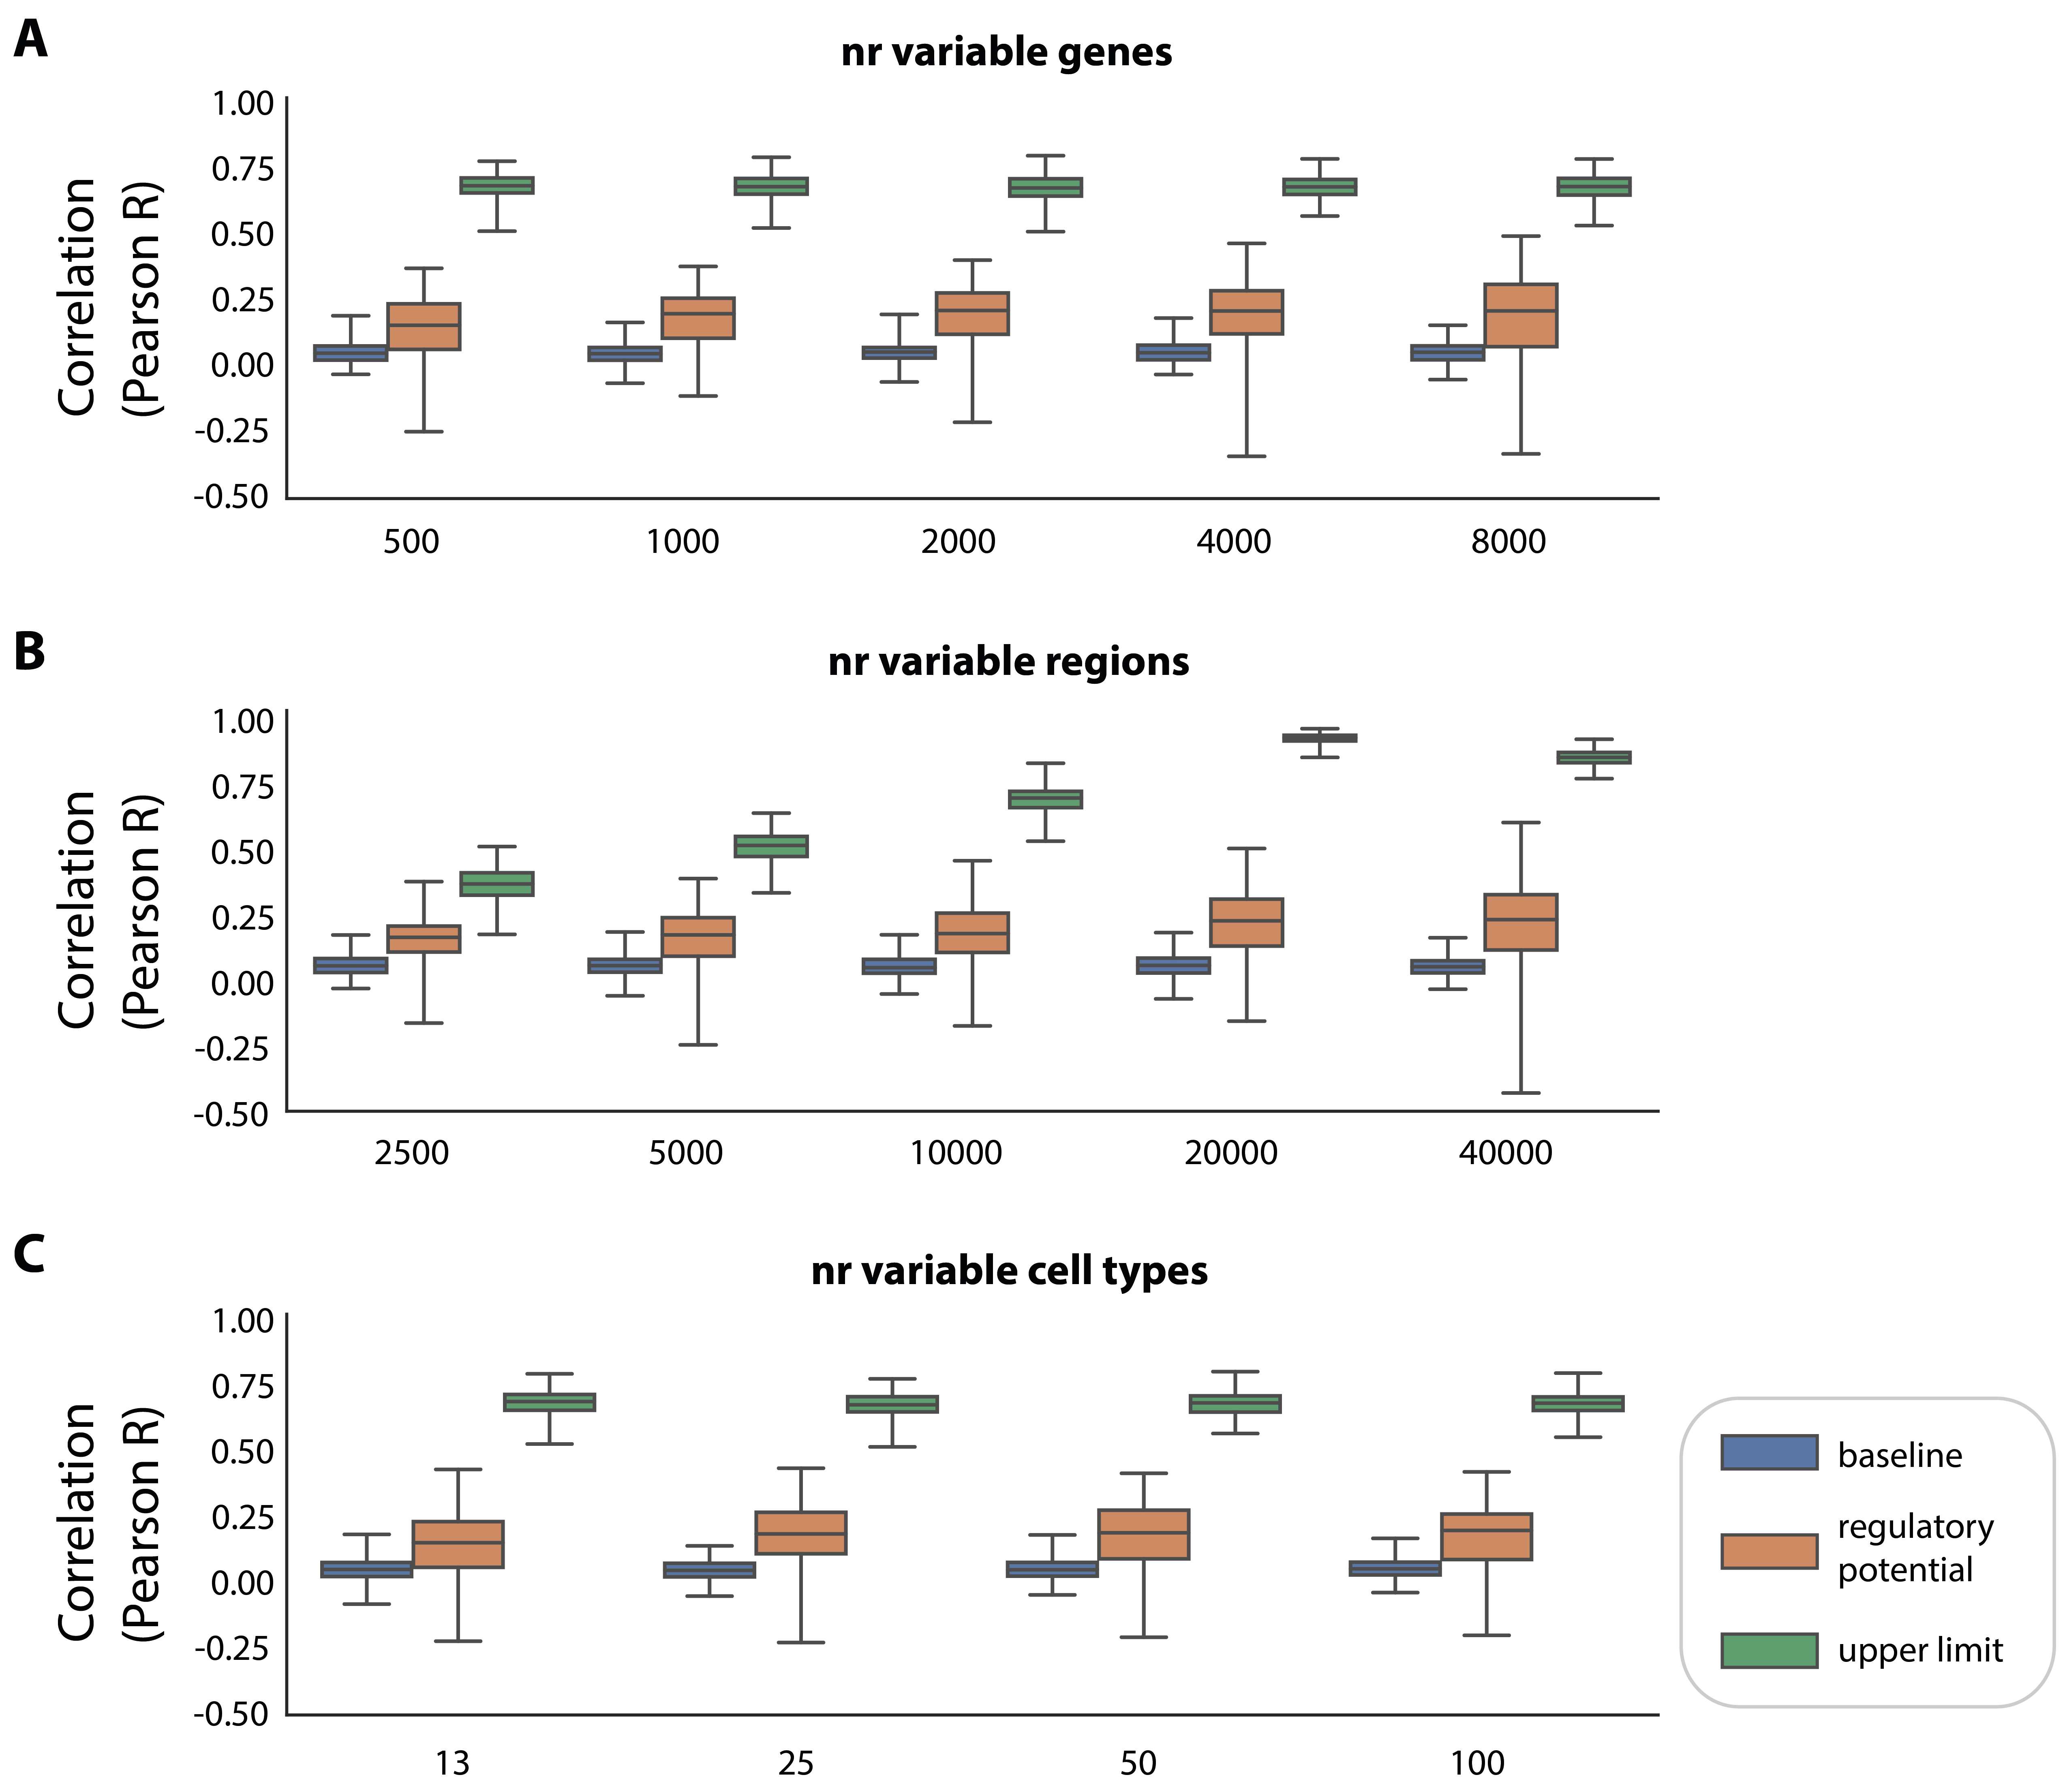
\includegraphics[width=\linewidth]{ch.scepia/imgs/BulkBenchmarks_MvS_Myriad_SuppFig1.png}
    \caption{}
    \label{fig:bulkbenchmark}
\end{figure}

\begin{figure}
    \centering
    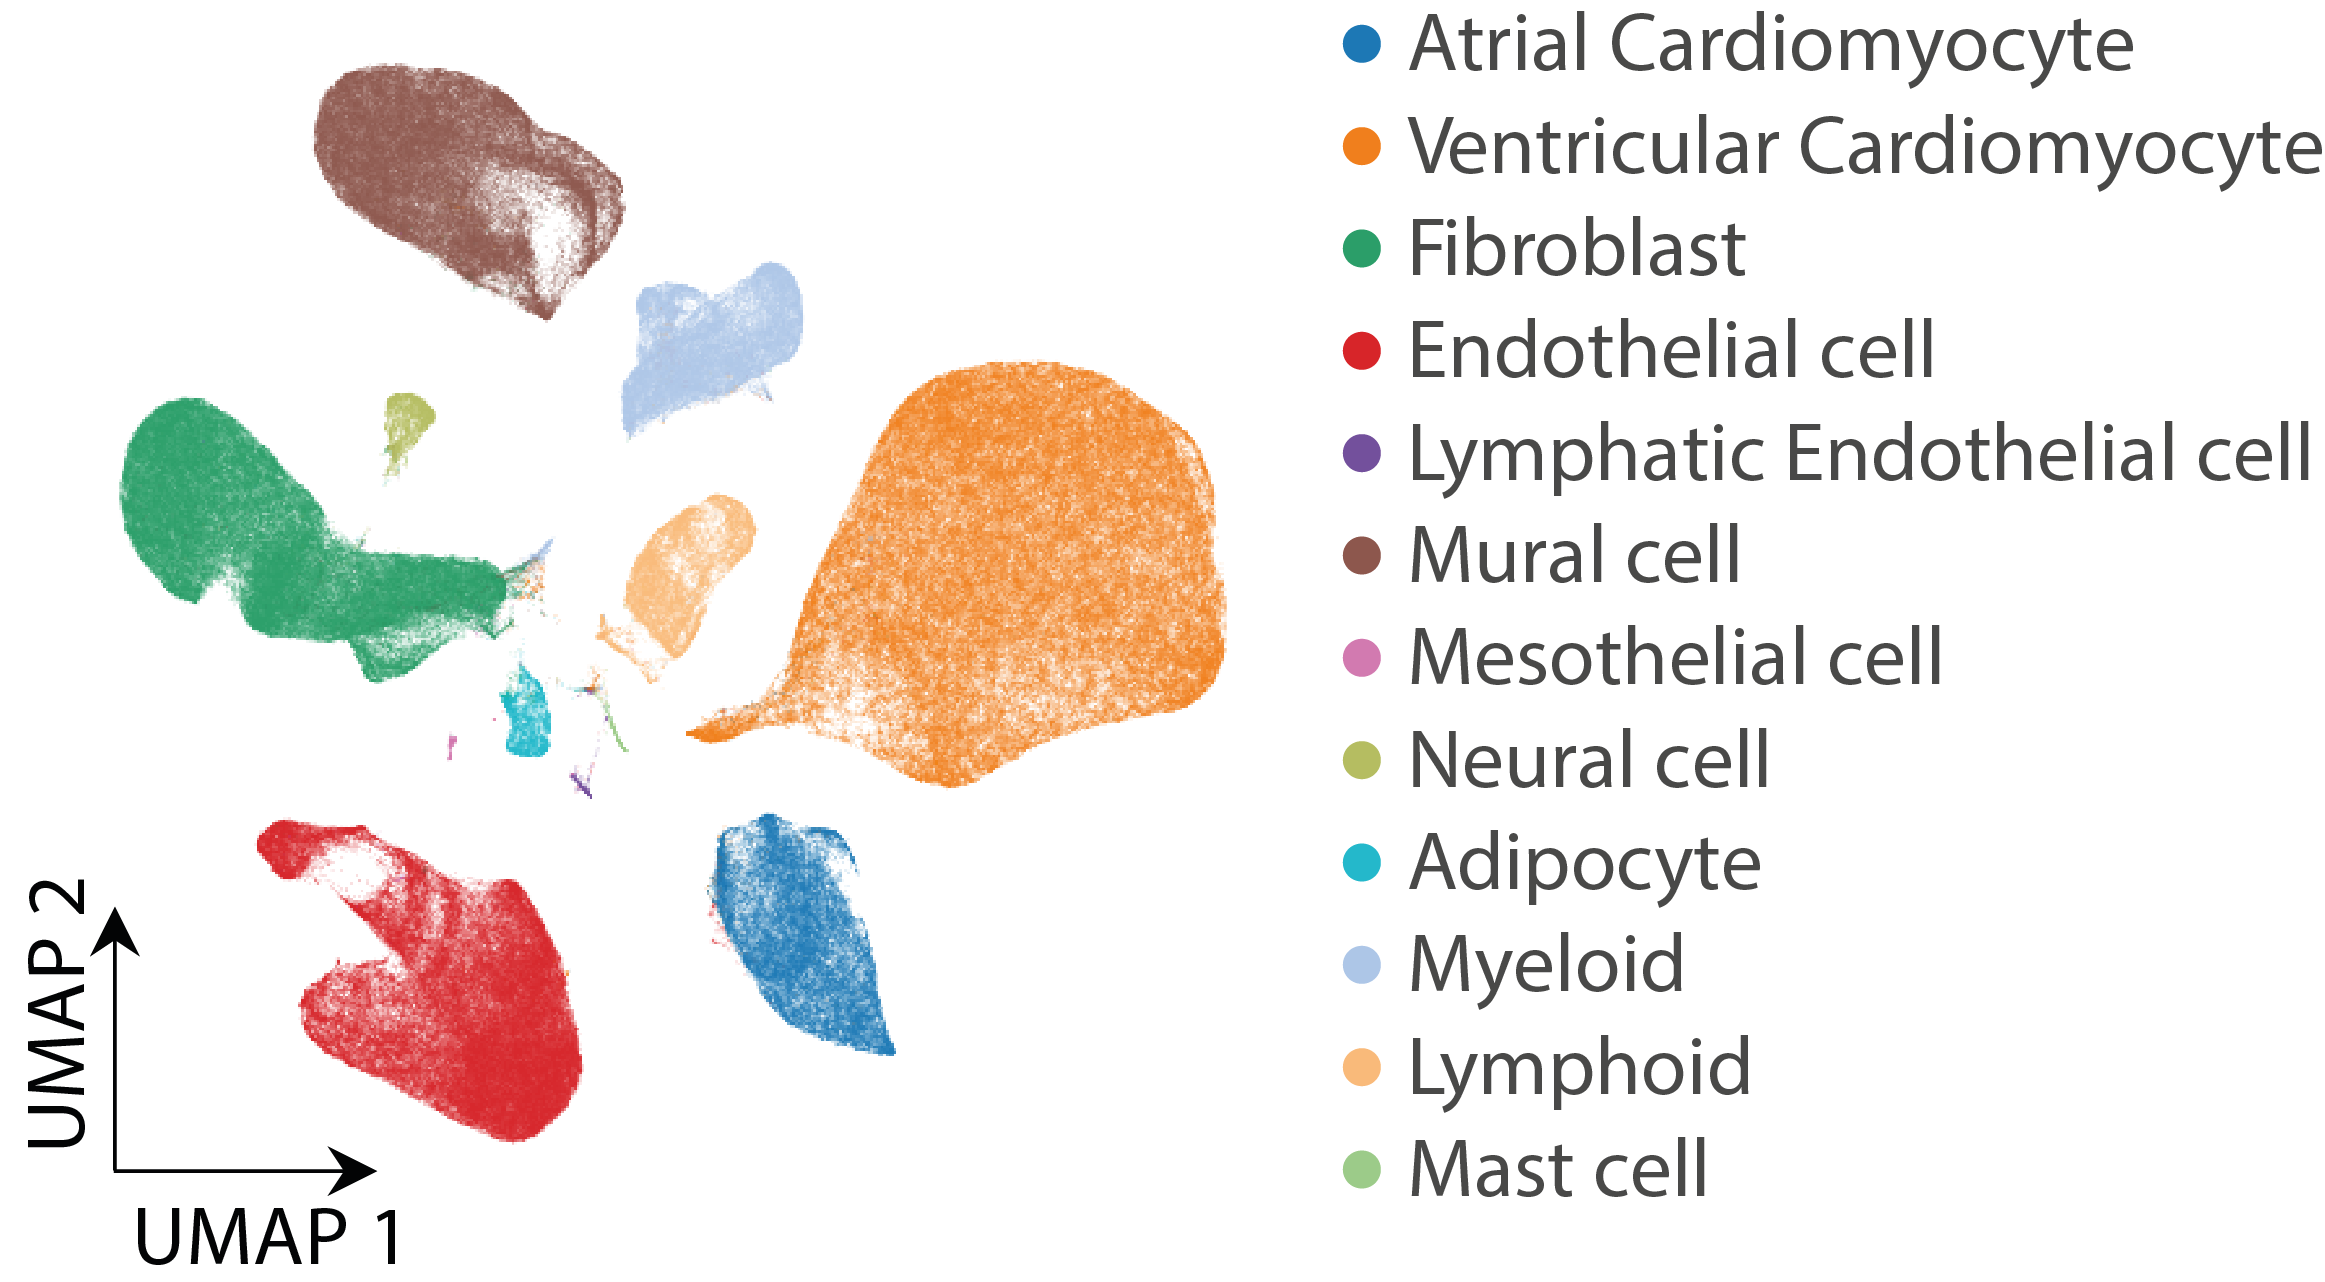
\includegraphics[width=\linewidth]{ch.scepia/imgs/SCEPIA_OriginalAnnotation_allCells_SuppFigAnno.png}
    \caption{Original annotation of cell types in the human Heart Cell Atlas (hHCA).}
    \label{fig:scepia_annotation1}
\end{figure}

\begin{figure}
    \centering
    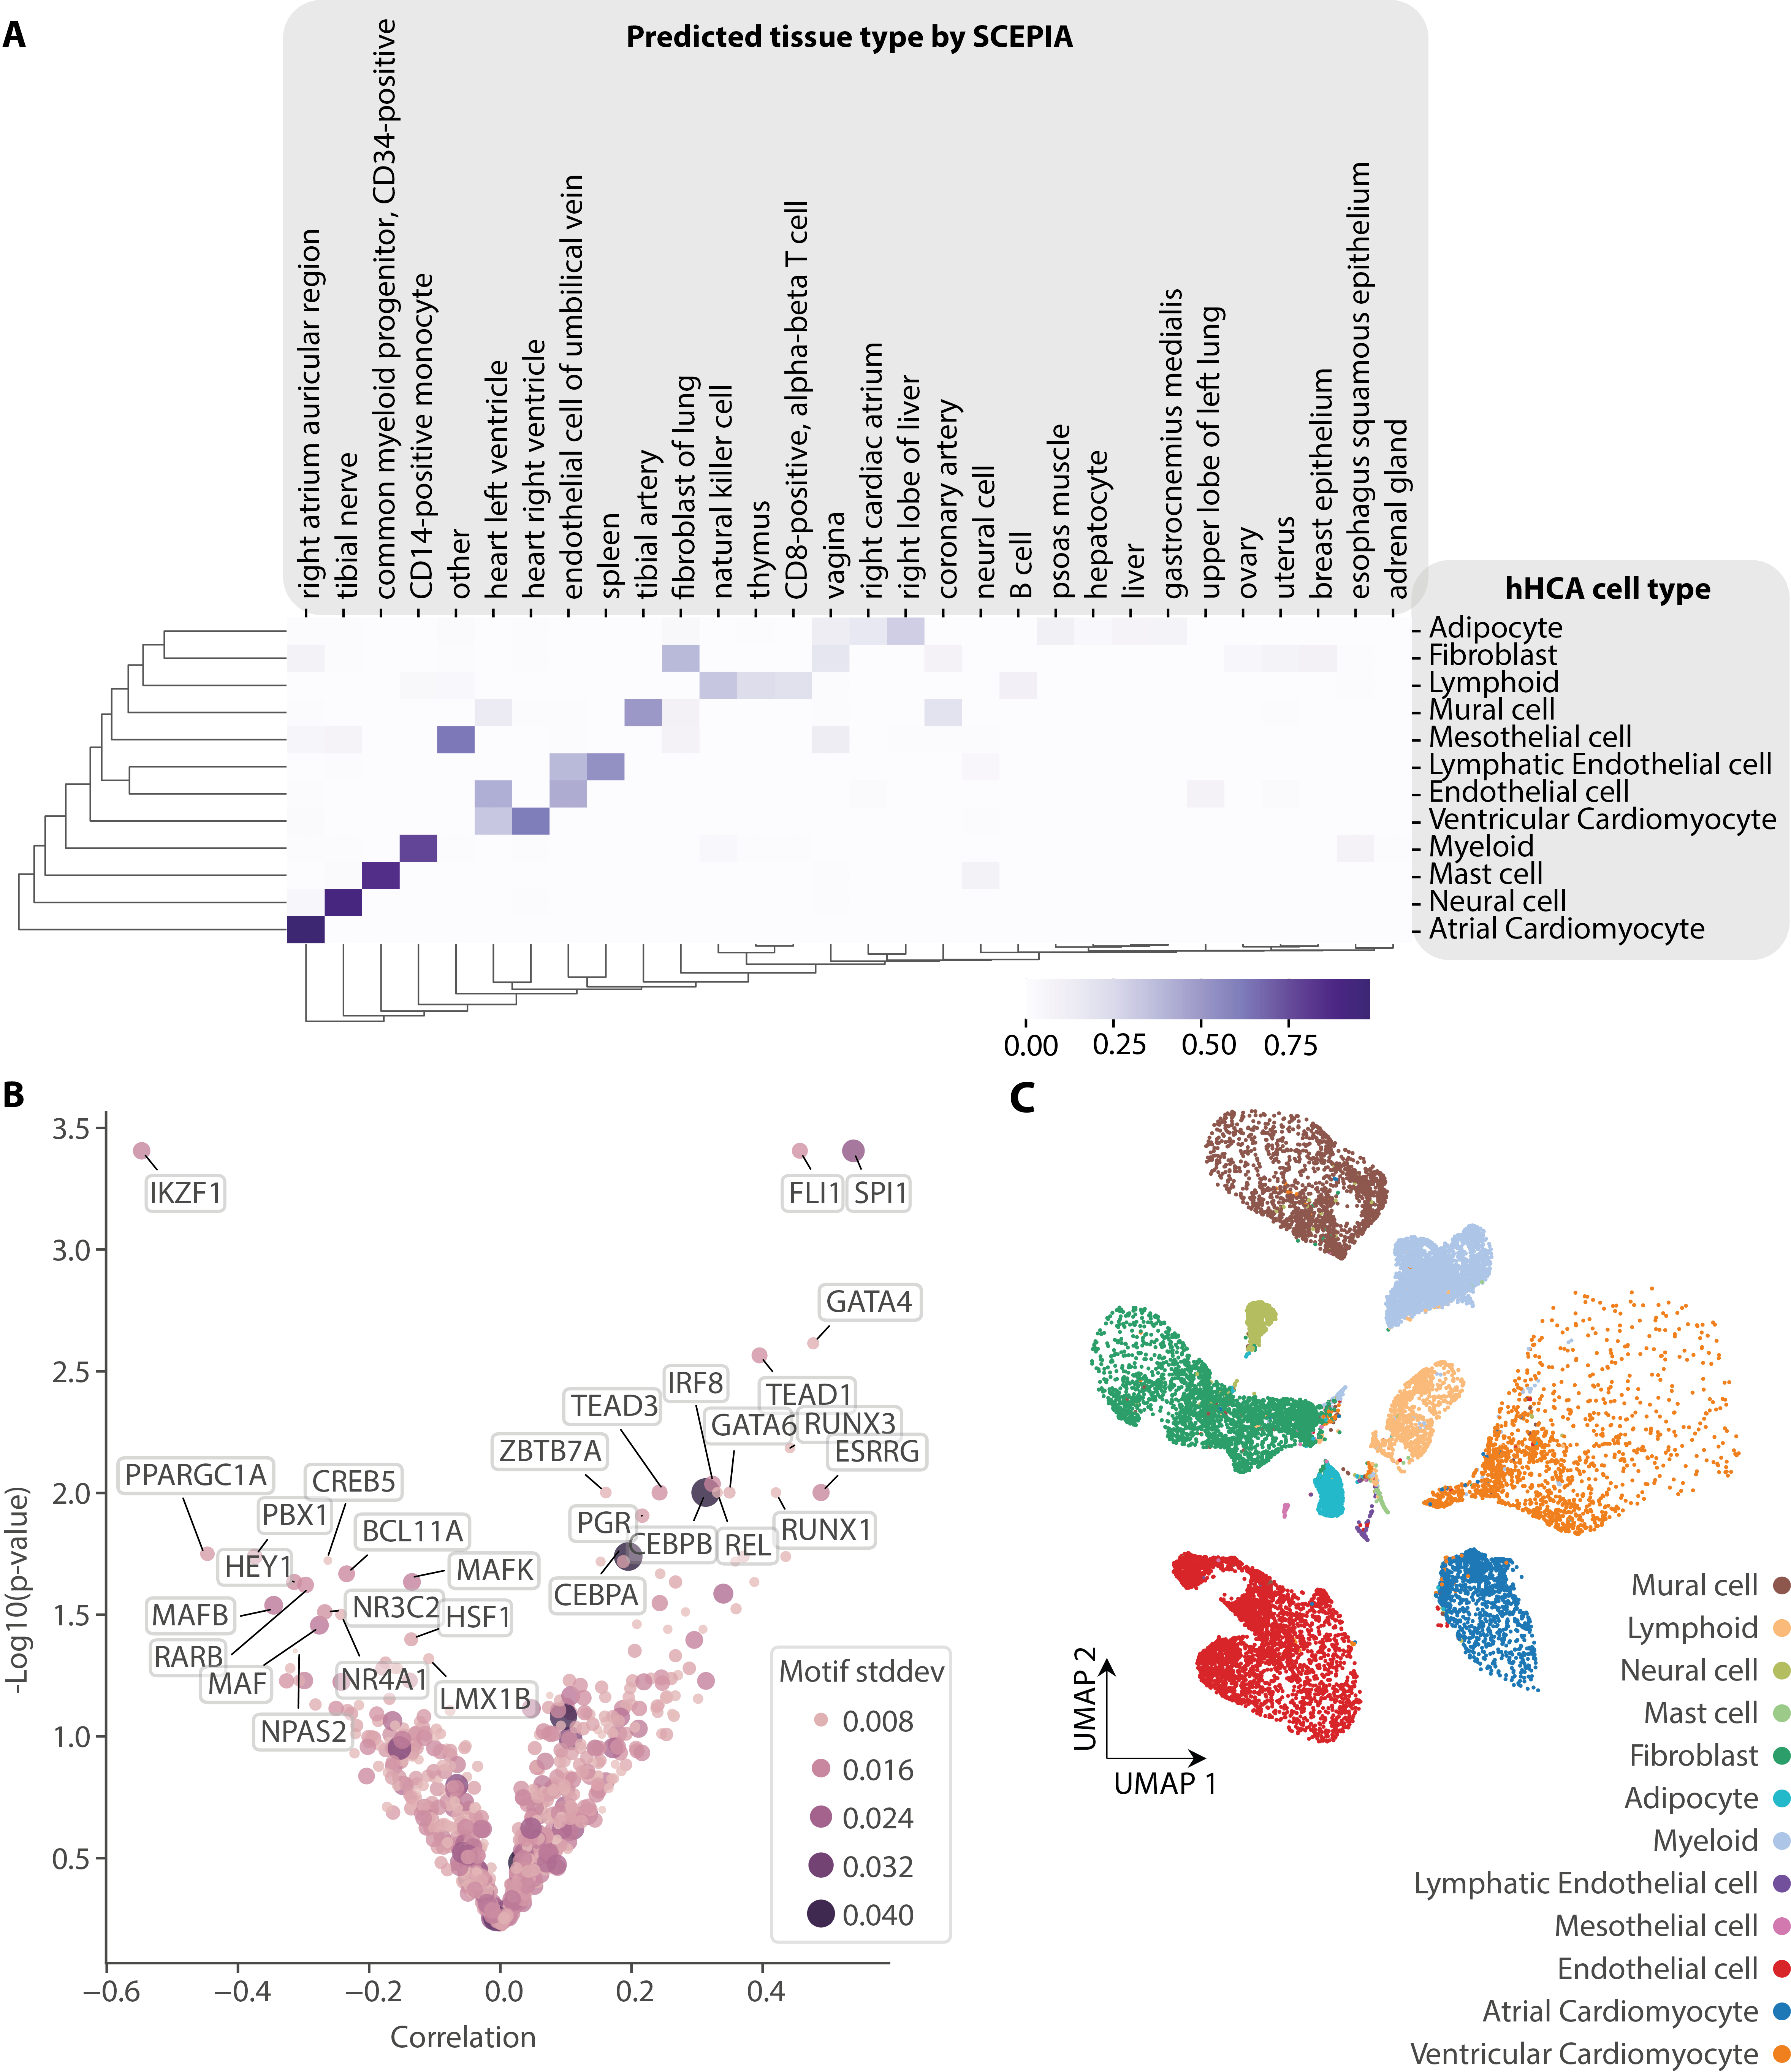
\includegraphics[width=\linewidth]{ch.scepia/imgs/SCEPIAGEOSKETCH_AllCells20000_Myriad_v3_SuppfigGeoAnno.png}
    \caption{SCEPIA run on geosketch of hHCA (A) SCEPIA annotation of clusters (B) Highest scoring motifs inferred with SCEPIA run on 700K cells (C) (placeholder XX) UMAP of 20K geosketch hHCA. }
    \label{fig:geoscepia_results}
\end{figure}

\begin{figure}
    \centering
    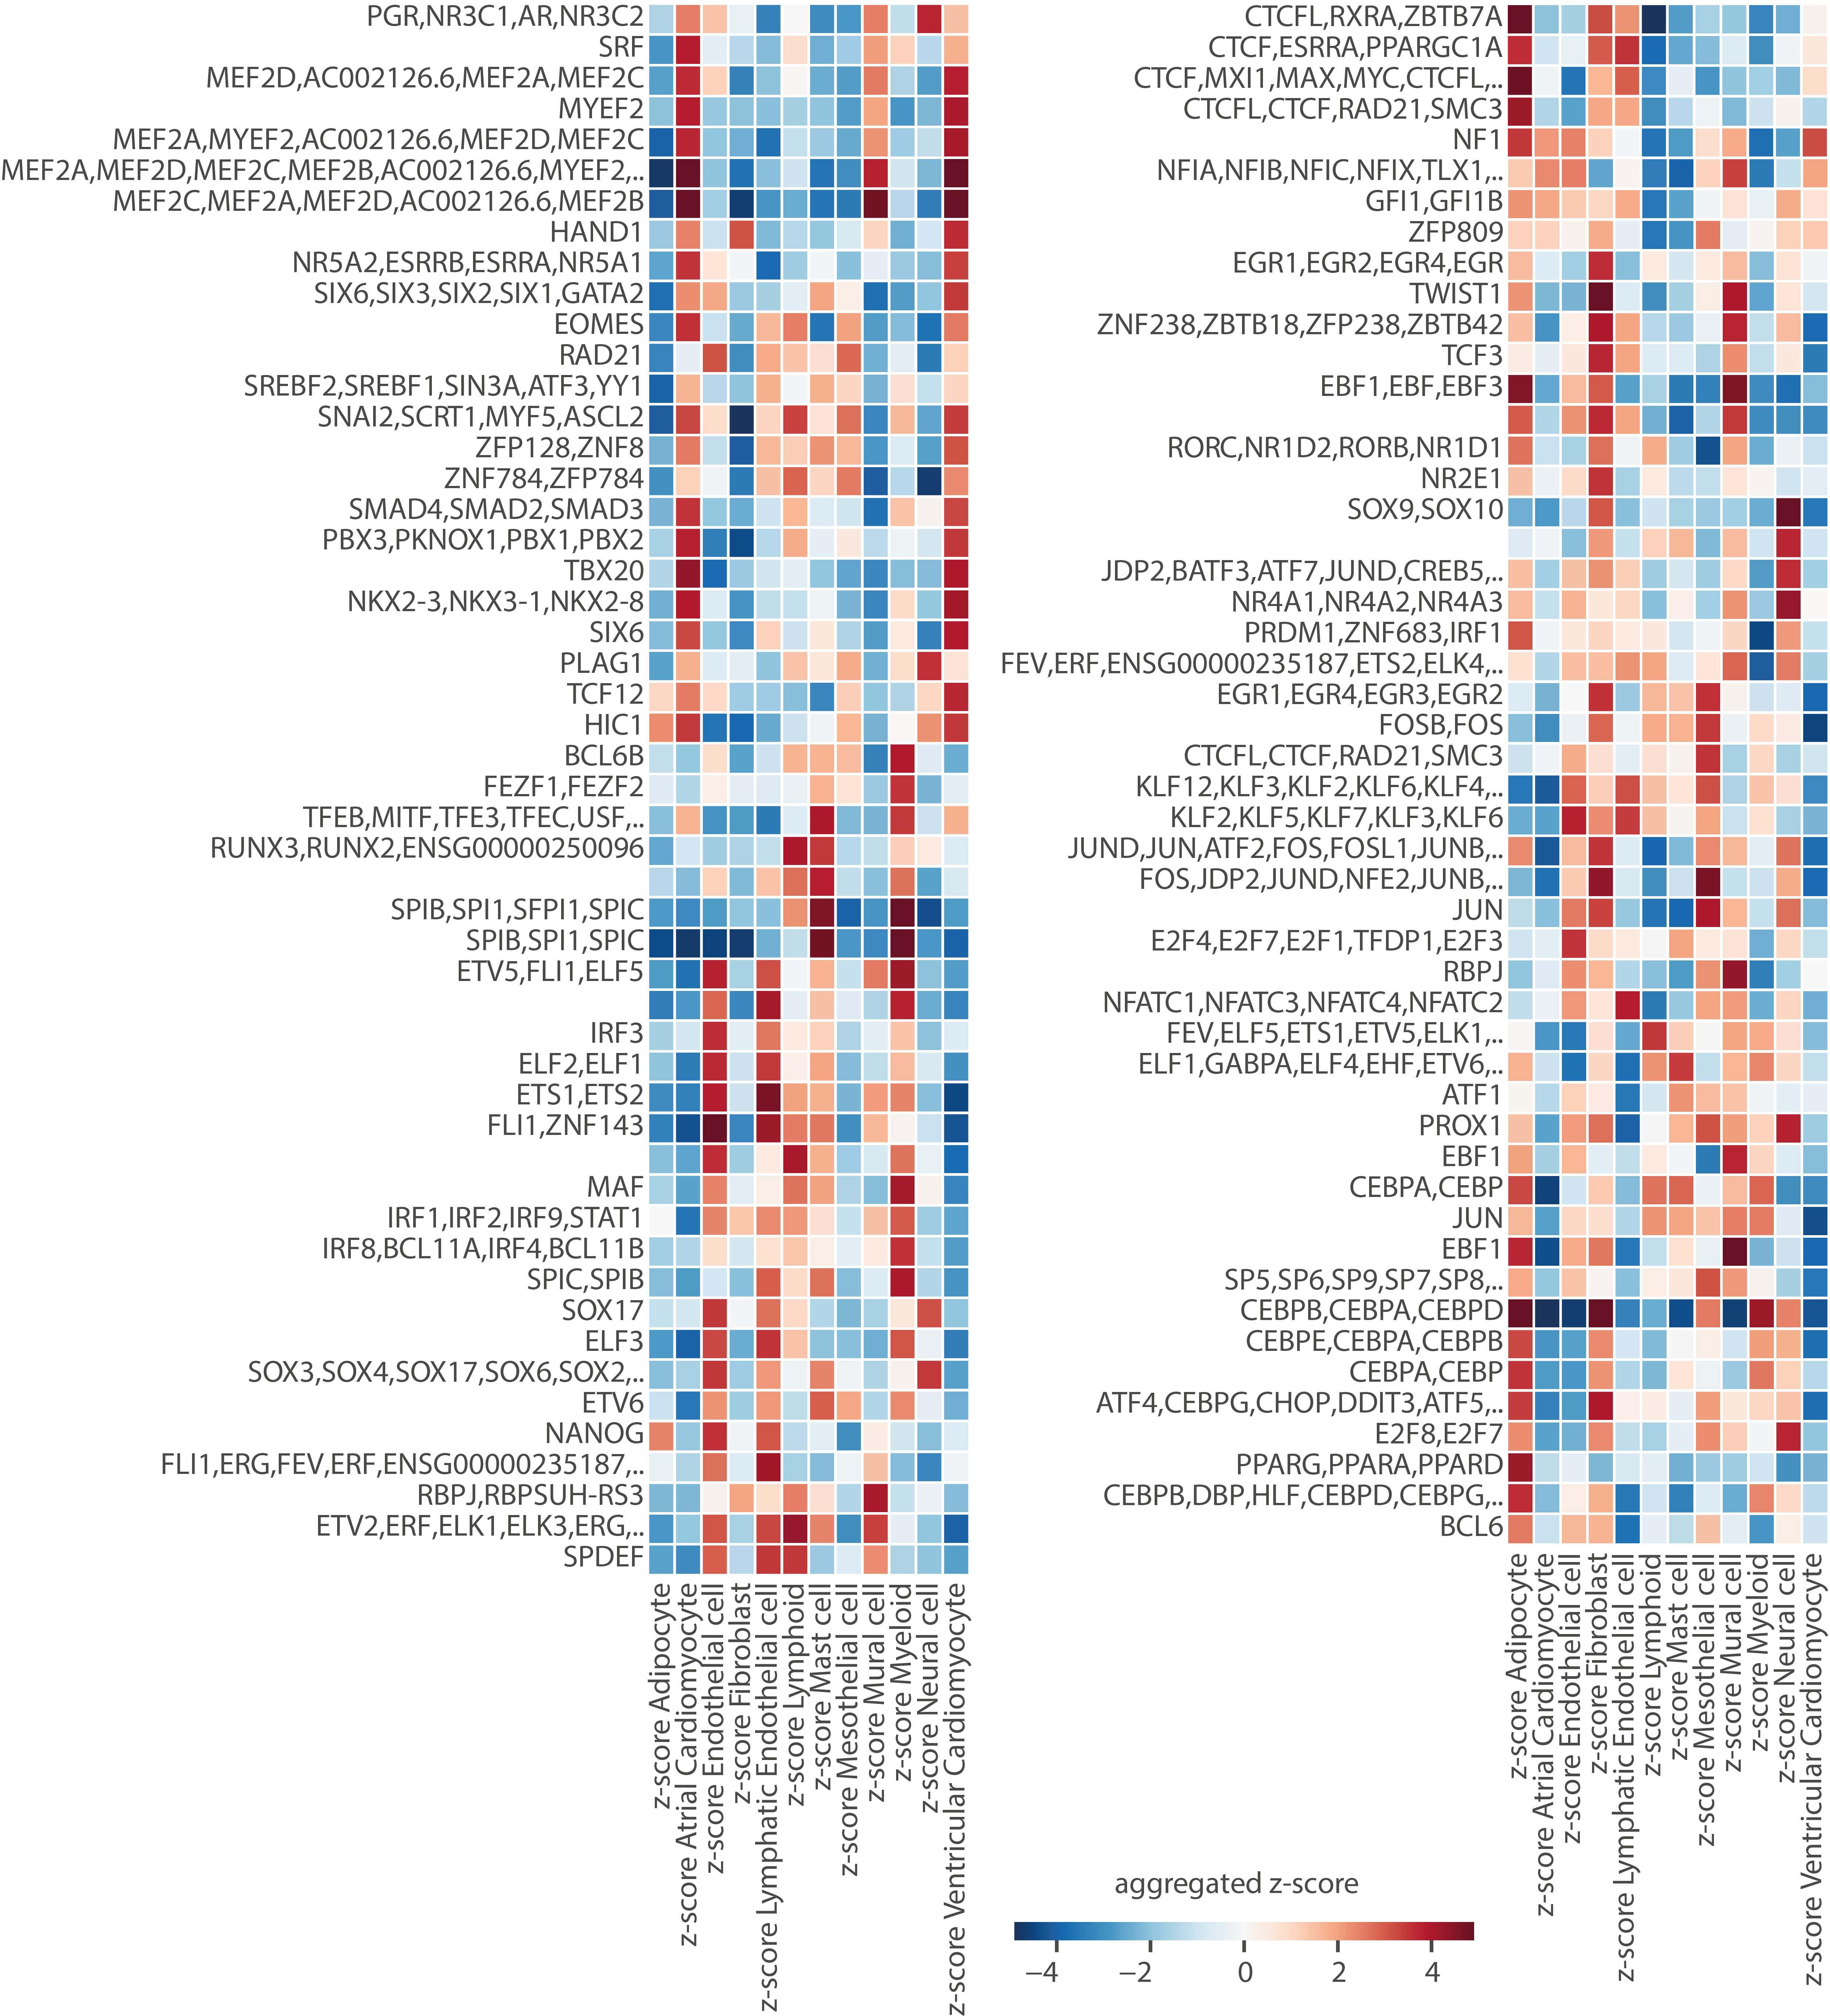
\includegraphics[width=\linewidth]{ch.scepia/imgs/Maelstrom_AllHitsAbove3.5_Myriad_SuppFigMaelstromHM.png}
    \caption{Maelstrom motif analysis output (z-score > 3.5) of the hHCA scATAC-seq cluster averages.}
    \label{fig:scepia_maelstromhm}
\end{figure}

\begin{figure}
    \centering
    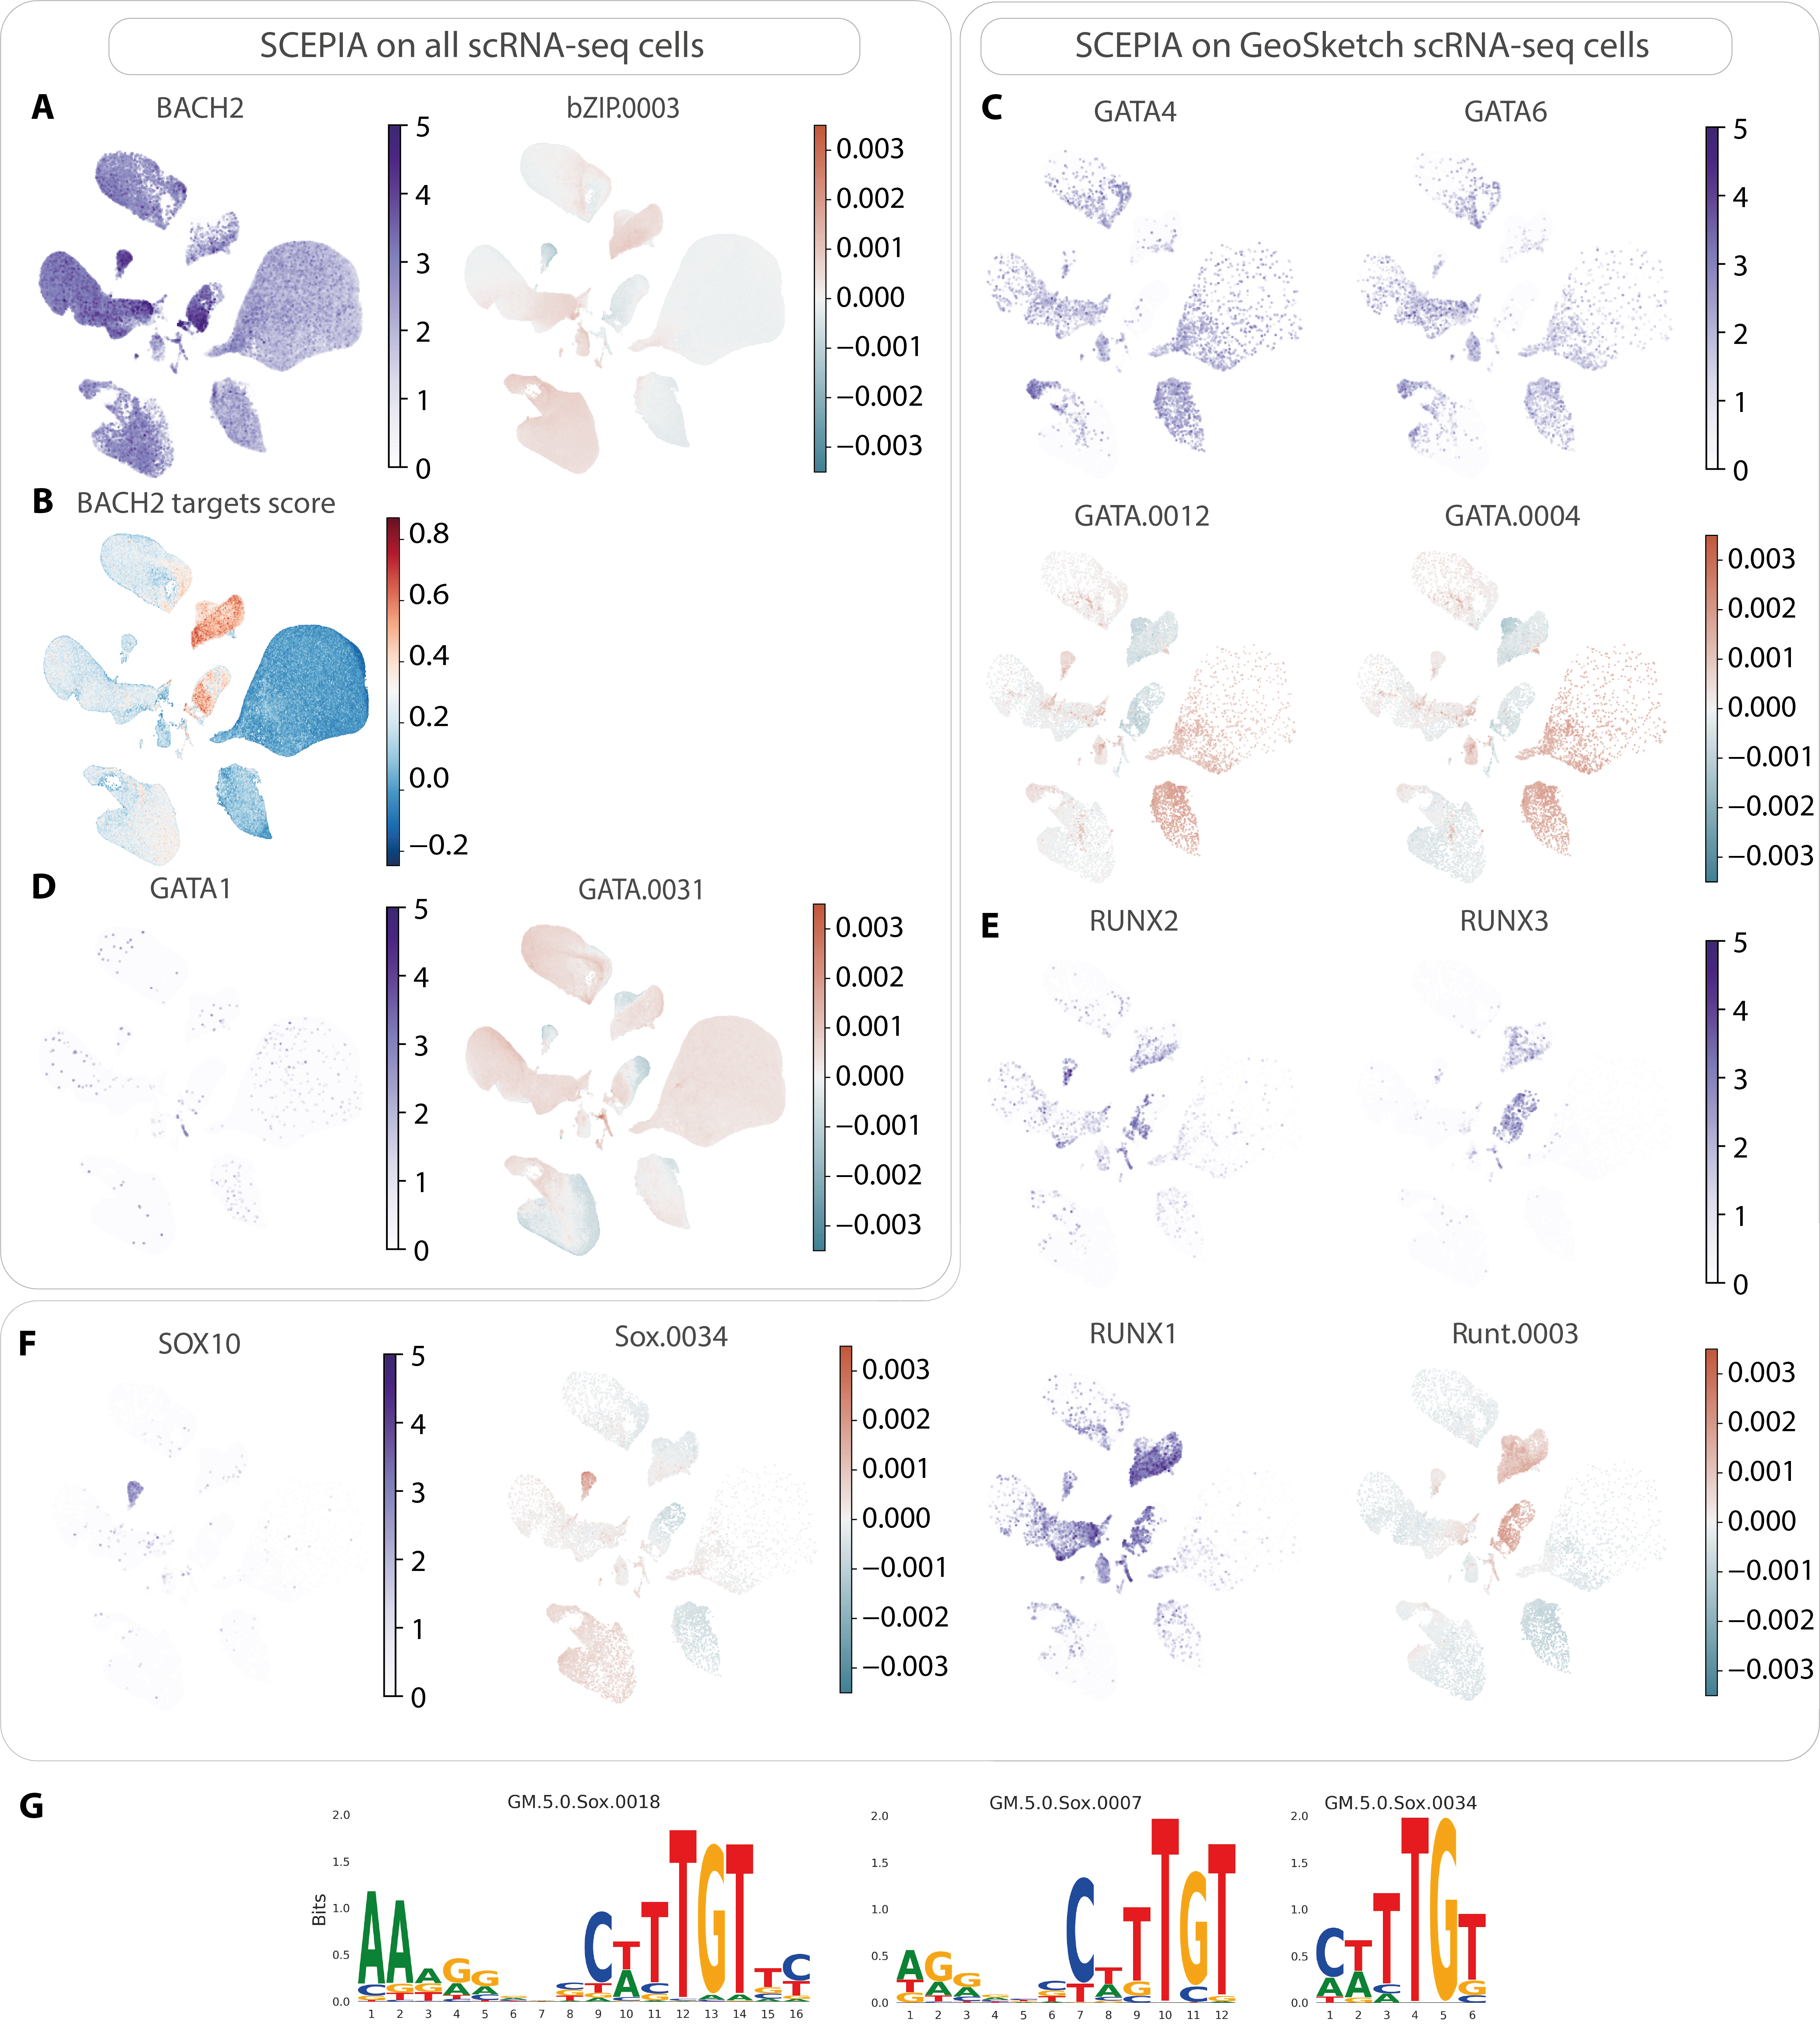
\includegraphics[height=1\linewidth]{ch.scepia/imgs/SCEPIA_SCEPIAGEO_BiologicalExamples_Myriad_v9_SuppFigFeatures1.png}
    \caption{Examples of SCEPIA and geosketch $+$ SCEPIA run \textcolor{red}{(\textbf{B}) Compound expression levels as calculated with scanpy\'s gene\_score function, of 57 BACH2 target genes. Target genes taken from ChIP Atlas (REFXX) results for BACH2 ChIPs in differring cell lines and "ChIP score" \> 100.}}
    \label{fig:scepia_features1}
\end{figure}

\begin{figure}
    \centering
    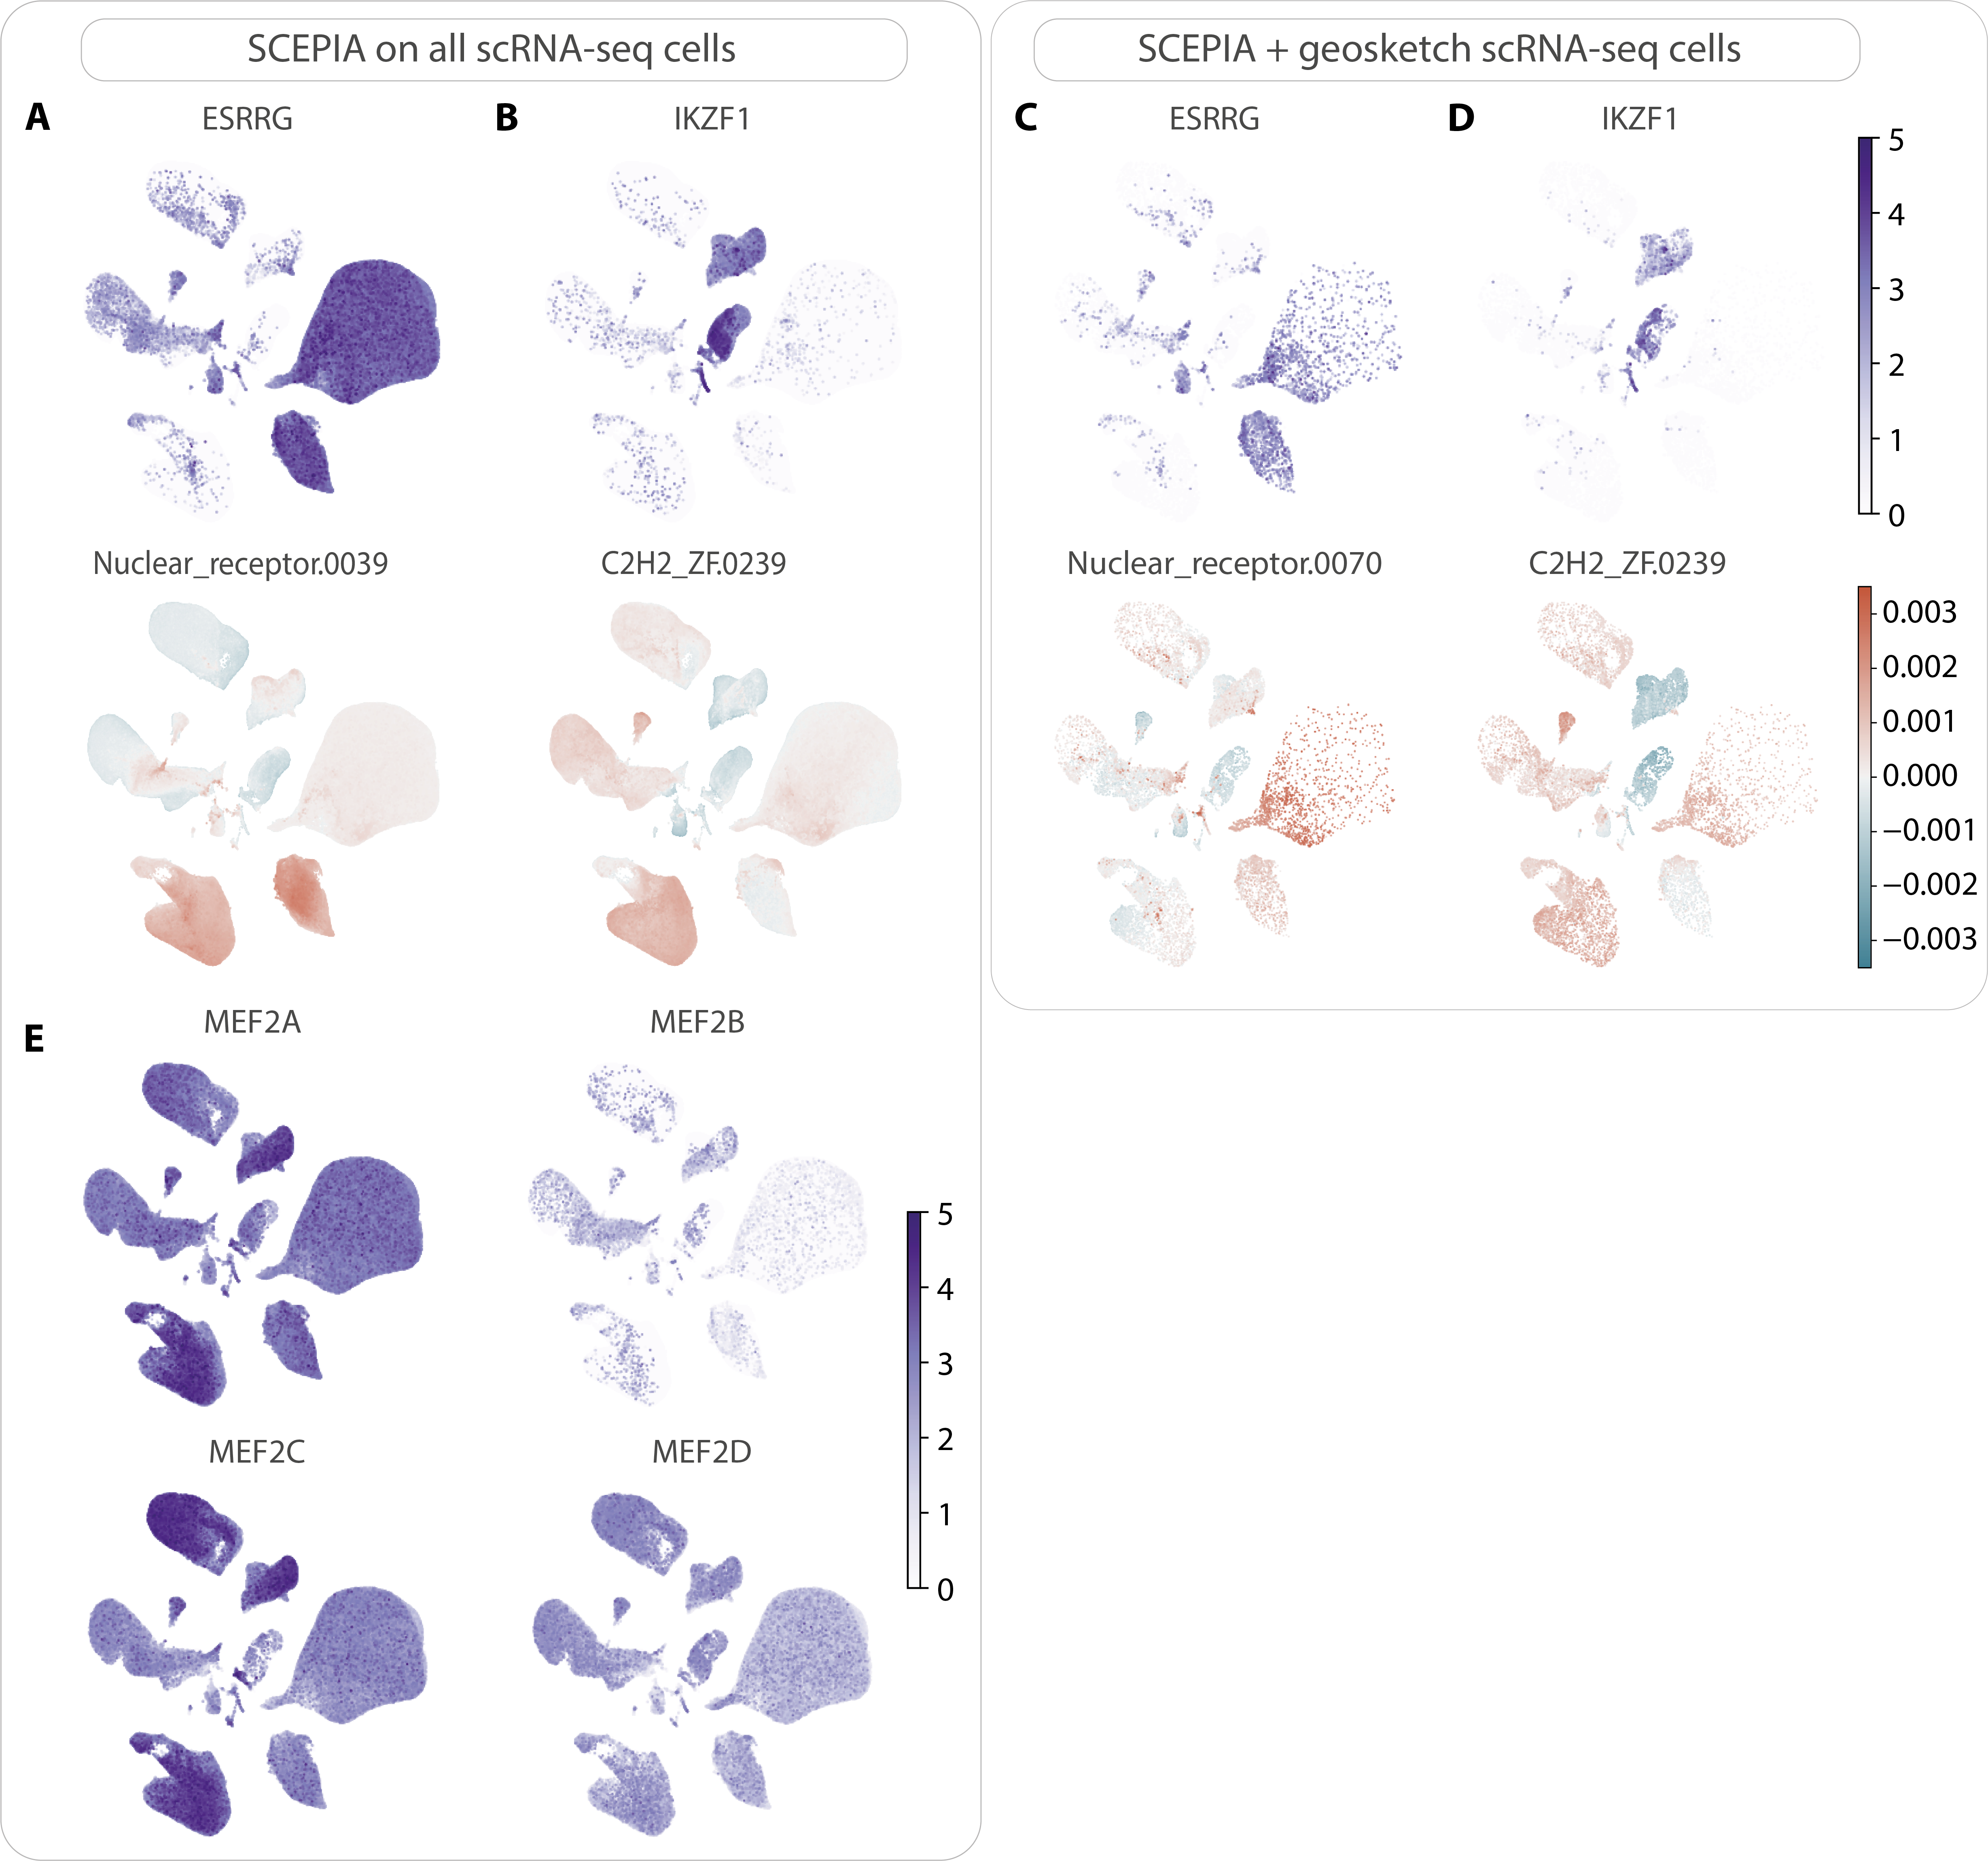
\includegraphics[height=0.666\linewidth]{ch.scepia/imgs/SCEPIA_SCEPIAGEO_BiologicalExamples_Myriad_v4_SuppFigFeatures2.png}
    \caption{Examples of SCEPIA and geosketch $+$ SCEPiA run}
    \label{fig:scepia_features2}
\end{figure}
